\section{Background}
\chead{\thesection. Background}

\subsection{The Central Dogma of Molecular Biology}

The central dogma of molecular biology defines the directional flow of genetic
information within a living system. This framework was first articulated by
Francis Crick in 1958 and has since been supported by decades of experimental
evidence \cite{centralDogma}. Crick's formulation distinguished three
sequential transfers that occur in all cellular organisms: DNA to DNA,
DNA to RNA, and RNA to protein. He also noted that other transfers, such as
protein to DNA, do not occur in nature.

Deoxyribonucleic acid (DNA) serves as the primary hereditary macromolecule. A
segment of DNA that encodes a functional product, such as a protein or
functional RNA, is defined as a \textit{gene}. The information stored in a gene
is first copied into messenger RNA (mRNA) in a process called
\textit{transcription}. The mRNA macromolecule is then decoded to assemble a
linear chain of amino acids, a protein, through \textit{translation}. This
directional flow is summarised as:

\[
\text{DNA} \xrightarrow{\text{transcription}} \text{mRNA} \xrightarrow{\text{translation}} \text{Protein}.
\]

The structure of these linear macromolecules is composed of residue monomers
(observe Fig.~\ref{fig:central_dogma} and
Appendix~\ref{appendix:aminoAcidLookup}). The central dogma ends at the primary
structure of a protein --- the linear sequence of amino acid residues. This
sequence determines the protein's higher-order structure and function, but
those properties are not directly encoded in the DNA. For computational protein
analysis, the primary structure is the central object of study, as
it can be directly compared across species and used to infer evolutionary and
functional relationships as well as the protein's spatial structure.

\begin{figure}[htbp]
  \centering
  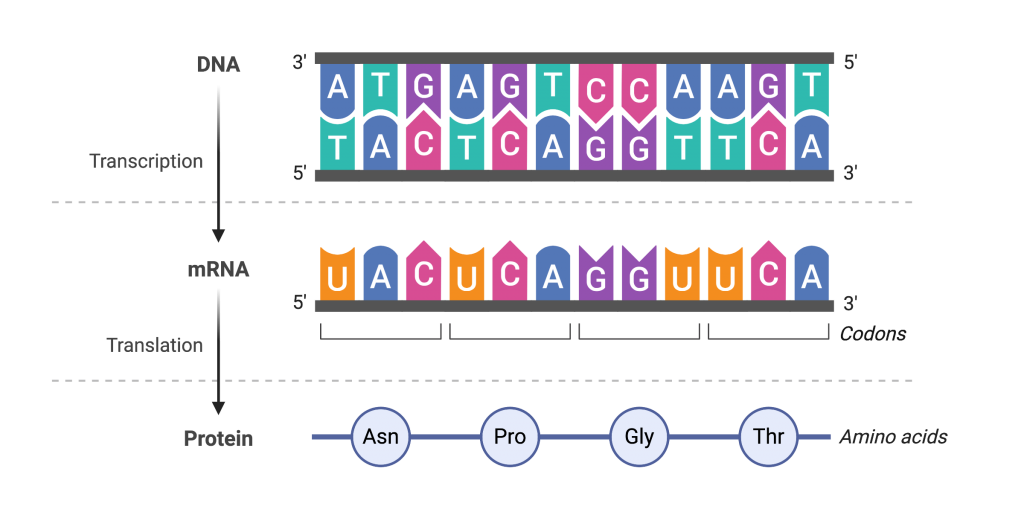
\includegraphics[width=1\linewidth]{asset/central_dogma.png}
  \caption{Flow of genetic information in a cellular organism. This image was created with BioRender (\href{https://www.biorender.com}{biorender.com}).}
  \label{fig:central_dogma}
\end{figure}

Proteins with similar sequences often share evolutionary origin or function ---
in the sense that they descend from a common ancestor, much like species in the
\textit{tree of life}. Grouping proteins by sequence similarity is therefore a
fundamental task in bioinformatics. This problem naturally maps to community
detection on weighted graphs where each protein becomes a vertex, edges connect
similar proteins, and clusters correspond to protein families.

\subsection{The Markov Cluster Algorithm}
\label{subsec:mcl}

MCL is a community detection algorithm that receives as input a weighted graph
and produces a set of communities (vertex clusters) by simulating a random
walk~\cite{mcl}. It is deterministic with respect to its input, therefore the
initial graph conditions yield a reproducible collection of output clusters.
Additionally, the algorithm is mathematically polished and well
studied~\cite{mclDetailed} while its algorithmic simplicity gives room
for computational optimization and scalability. For instance, the
implementation of HipMCL~\cite{hipmcl}, a high performance computing (HPC)
variant of MCL, is able to reliably process huge graphs comprised of at
least \(10^8\) vertices given that the compute cluster is sufficiently large.
MCL is capable of producing high quality clustering with a relatively low
computational cost and little need for tuning compared to other protein
clustering models. These properties collectively make MCL a suitable baseline
model for the task of biological sequence clustering, with a long track record
in a diverse set of tasks in biological sequence analyses~\cite{mclBrohee,
mclVlasblom, mclHaue, mclGibbons}.

Below is an algorithmic construction of MCL, applied on protein sequence data.
The purpose of this formulation is to provide a foundation, primarily for understanding
the computational complexity and memory requirements of the algorithm, which
are central to evaluating its scalability. At the same time, the formulation
highlights the stochastic mechanisms underlying MCL. We begin with a set of
definitions that establish the necessary groundwork.

\textbf{Definition 1}. For some \(n \in \mathbb{N}^*\), a \textit{weighted graph} is defined as \((\mathscr{V}, \mathcal{A})\), where \(\mathscr{V} = \{ v_i : i \in \{ 1, \dots, n \} \}\) holds all the graph's vertices and \(\mathcal{A}: \{ 1, \dots, n \}^2 \rightarrow \mathbb{R}\) is a square matrix where each row \(j\) and column \(k\) corresponds to vertices \(v_j\) and \(v_k\) respectively. The \(\mathcal{A}_{j,k}\) element of \(\mathcal{A}\) is the directed weight from the column \(k\) vertex to the row \(j\) vertex. \(\mathcal{A}\) is called the \textit{adjacency matrix}, and its elements satisfy the property
\[
  \forall j,k \in \{ 1, \dots, n \} \left( \mathcal{A}_{j, k} \geq 0 \ \wedge \ \mathcal{A}_{j, j} = 1 \right).
\]

\textbf{Definition 2}. For a weighted graph \((\mathscr{V}, \mathcal{A})\), if the adjacency matrix satisfies \(\mathcal{A}_{j, k} = \mathcal{A}_{k, j}\), then each element's weight is directionless, and \((\mathscr{V}, \mathcal{A})\) is called an \textit{undirected graph}.

\textbf{Definition 3}. For a weighted undirected graph \((\mathscr{V}, \mathcal{A})\), if \(\mathscr{V}\) is comprised of protein sequences and \(\mathcal{A}_{j,k}\) models the pairwise similarity of \(v_j, v_k \in \mathscr{V} \ ( j,k \in \mathbb{N}^* )\), then \((\mathscr{V}, \mathcal{A})\) is called a \textit{Protein Sequence Similarity Network} (\textit{PSSN}).

\textbf{Definition 4}. For a weighted graph \((\mathscr{V}, \mathcal{A})\), the \textit{Markov matrix} \(\mathcal{M}\) is a square matrix \(\mathcal{M}: \{ 1, \dots, n \}^2 \rightarrow [0, 1]\) where the value of cell \(\mathcal{M}_{j, k}\) semantically expresses the conditional \textit{probability of transition} from vertex \(v_k\) to \(v_j\) at the initial state with index $0$. Hence, \(\mathcal{M}_{j,k}\) acts as \(\mathcal{P}(v_j \ | \ v_k, \ \tau=0)\) in probabilistic literature.

\textbf{Remark}. In this case, the graph represents a stochastic system, where the \(k\) column of \(\mathcal{M}\) is normalized with respect to the \(k\) column of \(\mathcal{A}\) (observe Eq.~\ref{eq:markovMat}). Hence, the vector
\[
  \mathcal{M}_{\cdot, k} =
  \begin{pmatrix}
    \mathcal{P}(v_q \ | \ v_k, \ \tau=0) : q \in \{ 1, \dots, n \}
  \end{pmatrix}
\]
is a discrete probability distribution (PD).

For some set of protein sequences \(\mathscr{V}\), suppose that there exists a
pairwise similarity measure of that set's elements. Specifically, assume that
for each pair \(v_j, v_k \in \mathscr{V}\) there is some non-negative number
\(\mathcal{A}_{j,k} > 0\) encoding the pair's evolutionary similarity.
In the latter case, the adjacency
matrix \(\mathcal{A}\) quantifies a pairwise homology score between the
proteins \(v_k\) and \(v_j\) for all \(j, k \in \{ 1, \dots, n \}\). A
homologous protein collection descends from a common ancestral gene, and is
assumed to differ due to mutations, transcriptional\footnote{In genomics,
transcription is the process through which DNA generates the initial form of
RNA.} errors, or other sources of protein-sequence divergence.  On that basis,
the graph \((\mathscr{V}, \mathcal{A})\) is a PSSN representing the stochastic
system's initial state conditions at \textit{time} or \textit{step} \(\tau =
0\), and the task is to group together homologous proteins.

For proper usage of MCL and to preserve numerical stability throughout the internal iterations of the underlying random walk, \(\mathcal{A}\) must first be subjected to column-wise normalization. Thus, for every \(j,k \in \{ 1, \dots, n \}\), we set
\begin{align}
  \mathcal{M}_{j, k} := \dfrac{\mathcal{A}_{j, k}}{\sum_{q=1}^{n} \mathcal{A}_{q, k}}.
  \label{eq:markovMat}
\end{align}
Considering the fact that \(\mathcal{M} : \{ 1, \dots, n \}^2 \rightarrow [0, 1] \) is column normalized, each column represents a discrete PD, which in conjunction with the graph's independence from past states, implies that \(\mathcal{M}\) is a Markov matrix. Since each column of \(\mathcal{M}\) is a PD, its
\begin{align}
  \sum_{q=1}^{n} \mathcal{M}_{q, k} = 1
  \label{eq:sum1}
\end{align}
for all \(k \in \{ 1, \dots, n \}\).

The element \(\mathcal{M}_{j, k}\) is a measure of tendency for the vertex
\(v_k\) to land onto the vertex \(v_j\) after exactly one transition and can
thus be interpreted as the conditional probability \(\mathcal{P}(v_j \ | \ v_k,
\ \tau = 0)\). This tendency displays a directed \textit{flow of information} in
the graph. Also, because the measure is semantically tied to the protein pair's
evolutionary similarity, higher values express a higher statistical certainty
that the protein pair is homologous.
Subsequently, zero elements of \(\mathcal{M}\) correspond to disallowed vertex
transitions, representing non-homologous sequence pairs.

It is worth mentioning that \(\mathcal{A}\)'s symmetry does not ensure
\(\mathcal{M}\)'s symmetry because of the column-wise normalization performed
in Eq.~\ref{eq:markovMat}. The transition to the next state of the graph
depends entirely on its present state, making it independent from all previous
states. This is called the Markovian property of the stochastic system. This
property significantly simplifies the stochastic evolution of the graph towards
the next states, giving room for more interpretable and computationally
tractable approaches to the problem of protein clustering, while eliminating
the overhead of a more complicated mathematical structure and unnecessary
computational complexity.

Now we are ready to construct MCL in an iterative
form that underlies the aforementioned random walk. The integer \(\lambda \in
\mathbb{N}^*\) will denote the index of a specific random walk iteration.
Within that iteration, the stochastic system undergoes at least one state
transition --- through a parameter \(e\) which will be specified later. At
iteration \(\lambda\), MCL performs a transformation to some matrix
\(\mathcal{M}^{(\lambda-1)}\) called the \textit{transition matrix}. This
transformation produces another updated transition matrix\footnote{The notation
of the transition matrix \(\mathcal{M}^{(\lambda)}\) differs from
\(\mathcal{M}^{\lambda}\). In the former notation, the symbol \((\lambda)\)
wrapped in parentheses, represents a superscript, while in the latter the
integer \(\lambda\) represents an exponent of the Markov matrix
\(\mathcal{M}\).} \(\mathcal{M}^{(\lambda)}\).

This update simulates \textit{flow} in the graph, effectively pushing up the
probability of transition for sequence pairs with high correlation, while
decreasing that probability for pairs with low correlation. Given a sufficient
number of repetitions, the compounding effect of this repeated process on the
\(\mathcal{M}\) matrix eventually captures the strongest protein sequence edges
of similar proteins, and as a consequence, tightly connected proteins are
categorized into a collection of disjoint sub-regions that are called
communities or graph clusters (observe section 5 of \cite{mclDetailed}).

This process is outlined in the following pseudocode snippet:
\begin{plaintext}[showspaces=false, literate=]
Set parameters $e$ and $r$.
$\lambda := 1$
$\mathcal{M}^{(0)} := \mathcal{M}$
{
   $\texttt{w} := \mathcal{E}_e \mathcal{M}^{(\lambda-1)} \hspace*{0.00cm}$ # Expand.
   $\texttt{w} := \mathcal{Q} \texttt{w}                  \hspace*{1.121cm}$ # Prune.
   $\texttt{w} := \Gamma_r \texttt{w}                     \hspace*{1.044cm}$ # Inflate.
   $\mathcal{M}^{(\lambda)} := $ w
   $\lambda := \lambda + 1$
} Repeat while $\mathcal{M}^{(\lambda)}$ changes significantly compared to $\mathcal{M}^{(\lambda-1)}$.
\end{plaintext}

All details of the latter loop condition, as well as the operations of expansion \(\mathcal{E}_e\), pruning \(\mathcal{Q}\) and inflation \(\Gamma_r\) are detailed below. To complete the initialization of the iterative process, first set \(\lambda := 1\) and \(\mathcal{M}^{(0)}:=\mathcal{M}\).

\subsubsection{Expansion}

Expansion \(\mathcal{E}_e\) is an operator that subjects the probability matrix \(\mathcal{M}^{(\lambda)}\) to multi-step transitions in a single MCL iteration. Its parameter
\[
  e \ : \ e \in \mathbb{N} \ ( e \geq 2 )
\]
represents the number of state transitions applied per iteration. Say from iteration with index \(\lambda\) to \(\lambda+1\), the operation \(\mathcal{E}_e\) effectively expands the random walk's length, by incrementing the number of graph states by \(e-1\). Therefore, we have that
\begin{align}
  \mathcal{E}_e(\mathcal{M}^{(\lambda)}) = (\mathcal{M}^{(\lambda)})^e.
  \label{eq:expansion}
\end{align}
Since \(\mathcal{M}^{(\lambda)}\) is the transition matrix of the graph at iteration \(\lambda\), the statement
\begin{align}
  \mathcal{M}^{(\lambda)}_{j,k} = \mathcal{P}(v_j \ | \ v_k, \ \tau = (e-1) \cdot \lambda) 
  \label{eq:expProb}
\end{align}
holds for all \(j,k \in \{ 1, \dots, n \}\).

For lower exponent values \(e\), information propagates more smoothly in the graph after each subsequent MCL iteration. Hence, for \(e=2\) the transition matrix avoids supressing potentially valuable structural information before inflation can act.
In the official MCL implementation\footnote{\url{https://github.com/micans/mcl}.}, the value of the exponent \(e\) is set to \(2\). This is an appropriate choice in a computational setting since this setup prevents overshooting convergent solutions.

In this case, for any \(j,k \in \{ 1, \dots, n \}\), it's
\begin{align*}
  \mathcal{E}_{\epsilon}(\mathcal{M}^{(\lambda)})
  & \overset{(\ref{eq:expansion})}{=} \left(\left( \mathcal{M}^{(\lambda)} \right)^2\right)_{j, k}
  \\
  & = \sum_{q = 1}^{n} ( \mathcal{M}^{(\lambda)}_{j, q} \cdot \mathcal{M}^{(\lambda)}_{q, k} )
  \\
  & \overset{(\ref{eq:expProb})}{=} \sum_{q = 1}^{n} \left( \mathcal{P}(v_j \ | \ v_q, \ \tau = \lambda) \cdot \mathcal{P}(v_q \ | \ v_k, \ \tau = \lambda) \right). 
\end{align*}
Notice that expansion does not break the probabilities of \(\mathcal{M}^e\), since all elements of \(\mathcal{M}^e\) belong to the interval \([0, 1]\), and each matrix column sums to 1 (observe Appendix~\ref{appendix:proofExp}).

To preserve the output, we assign it in \texttt{w}, i.e., \(w := \mathcal{E}_e \mathcal{M}^{(\lambda)}\).

\subsubsection{Pruning}

After the expansion of the transition matrix \(\mathcal{M}^{(\lambda)}\), it is expected for many elements of the output matrix \texttt{w} to be extremely small.
These near-zero elements behave effectively like zero with negligible contribution to the dynamics of the random walk. On the other hand, sparsity is a desirable property that lowers the computational cost during subsequent iterations.
Thus, to increase graph sparsity and further leverage its computational benefit, all smaller value elements may be discarded based on an appropriate dynamic threshold \(f_k\) as a function of column index \(k\).

Since each column (node) carries its own PD per column \(\texttt{w}_{\cdot,k}\) with index \(k \in \{ 1, \dots, n \}\), the range of each column is unique and thus the threshold should be computed based on the statistical descriptors of the column's PD.
To respect this constraint, one way to model pruning is by first defining some constants \(a \in (0, 1]\) and \(b \in \{ 1, \dots, 8 \}\). Then set
\begin{align}
  f_k = a \cdot \text{ctr}(\texttt{w}_{\cdot, k}) \cdot \Big( \ 1 - b \cdot \big( \max( \texttt{w}_{\cdot, k} ) - \text{ctr}(\texttt{w}_{\cdot, k}) \big) \ \Big)
  \label{eq:pruningThreshold}
\end{align}
where
\[
  \text{ctr}(\texttt{w}_{\cdot, k}) = \Bigg( \sum_{j = 1}^{n} \texttt{w}_{j, k}^2 \Bigg)^{\frac{1}{2}}.
\]
Thus for a column \(k\), first compute the threshold \(f_k\) based on Eq.~\ref{eq:pruningThreshold}, and then for each row \(j\), if \( \texttt{w}_{j, k} < f_k \) is true then the element \( \texttt{w}_{j, k} \) is considered as trivial and through \textit{pruning} it gets discarded, i.e., \( \texttt{w}_{j, k} := 0 \).

\subsubsection{Inflation}

The role of inflation is to amplify edges that link node pairs belonging within a cluster (intra-cluster edges), while suppressing edges between nodes that belong to two different clusters (inter-cluster edges).
This happens through a straightforward element-wise exponentiation of the matrix \( \texttt{w} \), to the power of some parameter \( r \in \mathbb{R} \ (r > 1) \). Namely,
\[
  \Gamma_r \texttt{w} = ( \texttt{w}_{j, k}^{r} : j, k \in \{ 1, \dots, n \} ).
\]
Since MCL determines the number of clusters internally, it is important for the designer to have some control over that number. A way to control that number is by overriding the inflation parameter \(r\).
The selection of the exponent parameter \(r\) has an indirect influence on the \textit{granularity} of the final clusters. Granularity is a property of how fine grained the resulting clusters are, collectively. More specifically,
\begin{itemize}
  \item \(r \uparrow\) implies finer granularity : By increasing \(r\), we expect finer grained cluster collection, hence a higher number of smaller clusters.
  \item \(r \downarrow\) implies coarser granularity : By decreasing \(r\), we expect coarser grained cluster collection, hence a lower number of larger clusters.
\end{itemize}
Usually, the selection \(r\) is bounded in the interval \([1.2, 5]\).

Generally, inflation provides a simple yet effective tuning mechanism for exploring the network's community structure at different resolutions.

\subsubsection[Stochasticity Reconstruction \& \ Termination Condition]{Stochasticity Reconstruction \& Termination Condition}

Matrix \(\texttt{w}\) is not necessarily a transition matrix given the aforementioned transformations that it was subjected to.
This is a problem if we want to continue applying these transformations iteratively since at this point, \(\texttt{w}\) has lost the probabilistic structure that conveys the weighted graph's flow.
That is why, as a final step of iteration \(\lambda\), the matrix \(\texttt{w}\) is converted into a transition matrix through the following normalization. Thus, we now set the updated transition matrix as
\begin{align*}
  \mathcal{M}^{(\lambda+1)}_{j,k} := \texttt{w}_{j,k} \Big{/} \sum_{q=1}^{n} \texttt{w}_{q,k}
\end{align*}
for all \(j,k \in \{ 1, \dots, n \}\).

This entire process is practically repeated up to some finite iteration \(\lambda_0\), in which the update from \(\mathcal{M}^{(\lambda_0-1)}\) to \(\mathcal{M}^{(\lambda_0)}\) is insignificant with trivial changes on the latter stochastic matrix at \(\lambda_0\) compared to the preceding one at iteration \(\lambda_0-1\). The termination condition that defines \(\lambda_0\) could be implemented as follows
\begin{align}
  \left\| \mathcal{M}^{(\lambda)} - \mathcal{M}^{(\lambda-1)} \right\|_\text{F} < \epsilon_0 \cdot n^2
  \label{eq:term}
\end{align}
for some small enough value \(\epsilon_0 \in \mathbb{R} \ ( \epsilon_0 > 0)\), where \(\| \cdot \|_\text{F}\) is the Frobenius norm defined as
\[
  \left\| \mathcal{X} \right\|_\text{F} := \Bigg( \sum_{j=1}^{n} \sum_{k=1}^{n} \left| \mathcal{X}_{j,k} \right|^2 \Bigg)^{\frac{1}{2}}.
\]
In a computational setting, the loop of MCL will terminate when Eq.~\ref{eq:term} is satisfied for the first time.
According to the rigorous analysis performed in \cite{mclDetailed}, the
sequence \(\lambda \mapsto \mathcal{M}^{(\lambda)}\) can converge fast to some
block diagonal real matrix \(\lim_{\lambda \rightarrow \infty}
\mathcal{M}^{(\lambda)}\), given that the inflation parameter \(r\) is set to a
high enough value. The said matrix regions are tightly connected, typically
exhibiting a much higher sparsity compared to \(\mathcal{A}\). This result
allows us to safely assume the existence of some relatively low \(\lambda_0\)
that leads to a collection of clusters.

An example of an asymptotic transition matrix follows below:
\[
  \lim_{\lambda \rightarrow \infty} \mathcal{M}^{(\lambda)}
  \\
  =
  \begin{pmatrix}
0.34 & 0.32 & 0.33 & 0 & 0 & 0 & 0 & 0 & 0 & 0 & 0 & 0 \\
0.32 & 0.36 & 0.35 & 0 & 0 & 0 & 0 & 0 & 0 & 0 & 0 & 0 \\
0.33 & 0.32 & 0.32 & 0 & 0 & 0 & 0 & 0 & 0 & 0 & 0 & 0 \\
0 & 0 & 0 & 0.34 & 0.34 & 0.33 & 0.25 & 0 & 0 & 0 & 0 & 0 \\
0 & 0 & 0 & 0.34 & 0.37 & 0.32 & 0.26 & 0 & 0 & 0 & 0 & 0 \\
0 & 0 & 0 & 0.33 & 0.35 & 0.35 & 0.27 & 0 & 0 & 0 & 0 & 0 \\
0 & 0 & 0 & 0.25 & 0.21 & 0.32 & 0.32 & 0 & 0 & 0 & 0 & 0 \\
0 & 0 & 0 & 0 & 0 & 0 & 0 & 0.51 & 0.49 & 0 & 0 & 0 \\
0 & 0 & 0 & 0 & 0 & 0 & 0 & 0.48 & 0.52 & 0 & 0 & 0 \\
0 & 0 & 0 & 0 & 0 & 0 & 0 & 0 & 0 & 1 & 0 & 0 \\
0 & 0 & 0 & 0 & 0 & 0 & 0 & 0 & 0 & 0 & 0.53 & 0.47 \\
0 & 0 & 0 & 0 & 0 & 0 & 0 & 0 & 0 & 0 & 0.47 & 0.53
  \end{pmatrix}.
\]
In the example above, consider only the non-trivial blocks found in the
diagonal. Each such square submatrix represents an isolated region
corresponding to a distinct cluster. As it can be observed, there are five such
blocks in total. That is what the output of MCL may look like. Another example
can be observed in Fig.~\ref{fig:mcl_iter}, showcasing how MCL internally
processes an entangled graph starting from some complicated and relatively
sparse transition matrix \(\mathcal{M}\), until it successfully converges to a
disjoint collection of distinct regions without the initial noise of the weaker
edges.

\begin{figure}[htbp]

  \captionsetup[subfigure]{font=scriptsize}

  \vspace{-0.3cm}

  \hspace{0.5cm}
  \begin{subfigure}{0.40\linewidth}
    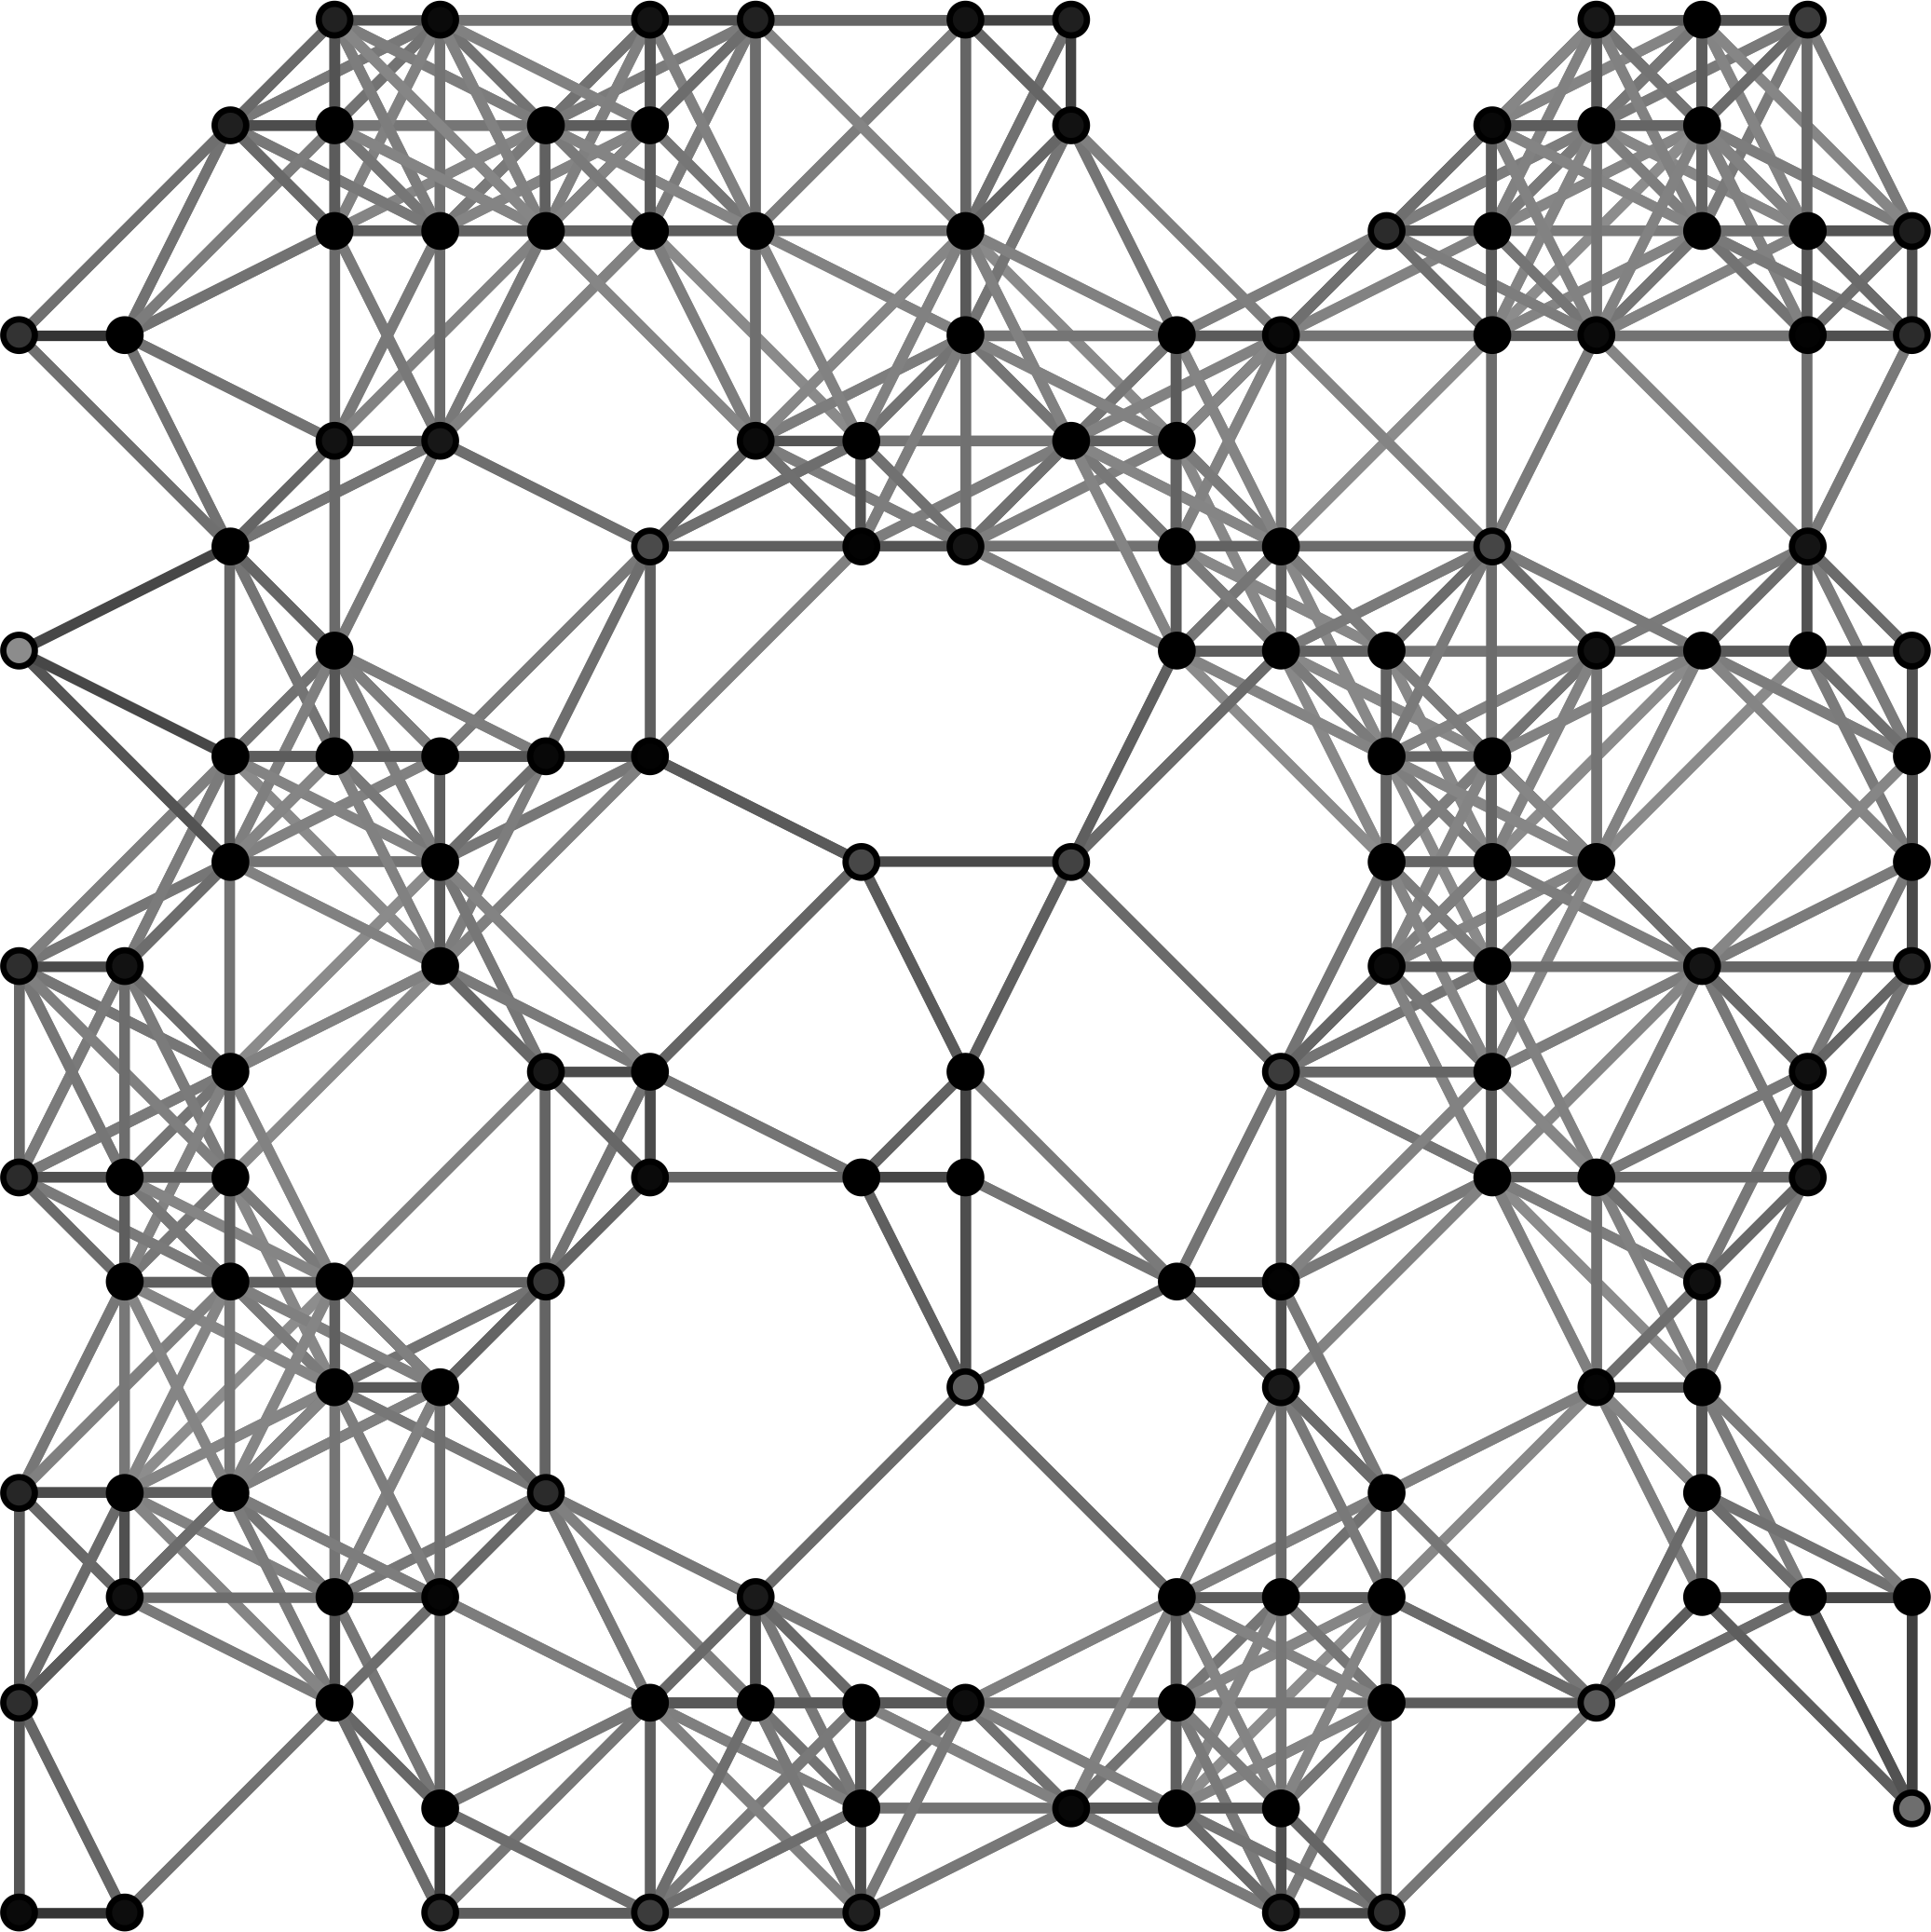
\includegraphics[width=\linewidth]{asset/mcl_iter_0.png}
    \subcaption{The pre-processed input graph \((\mathscr{V}, \mathcal{M})\) where \(\mathcal{M}\) is some sparse Markov matrix.}
    \label{fig:mcl_iter_1}
  \end{subfigure}
  \hfill
  \begin{subfigure}{0.40\linewidth}
    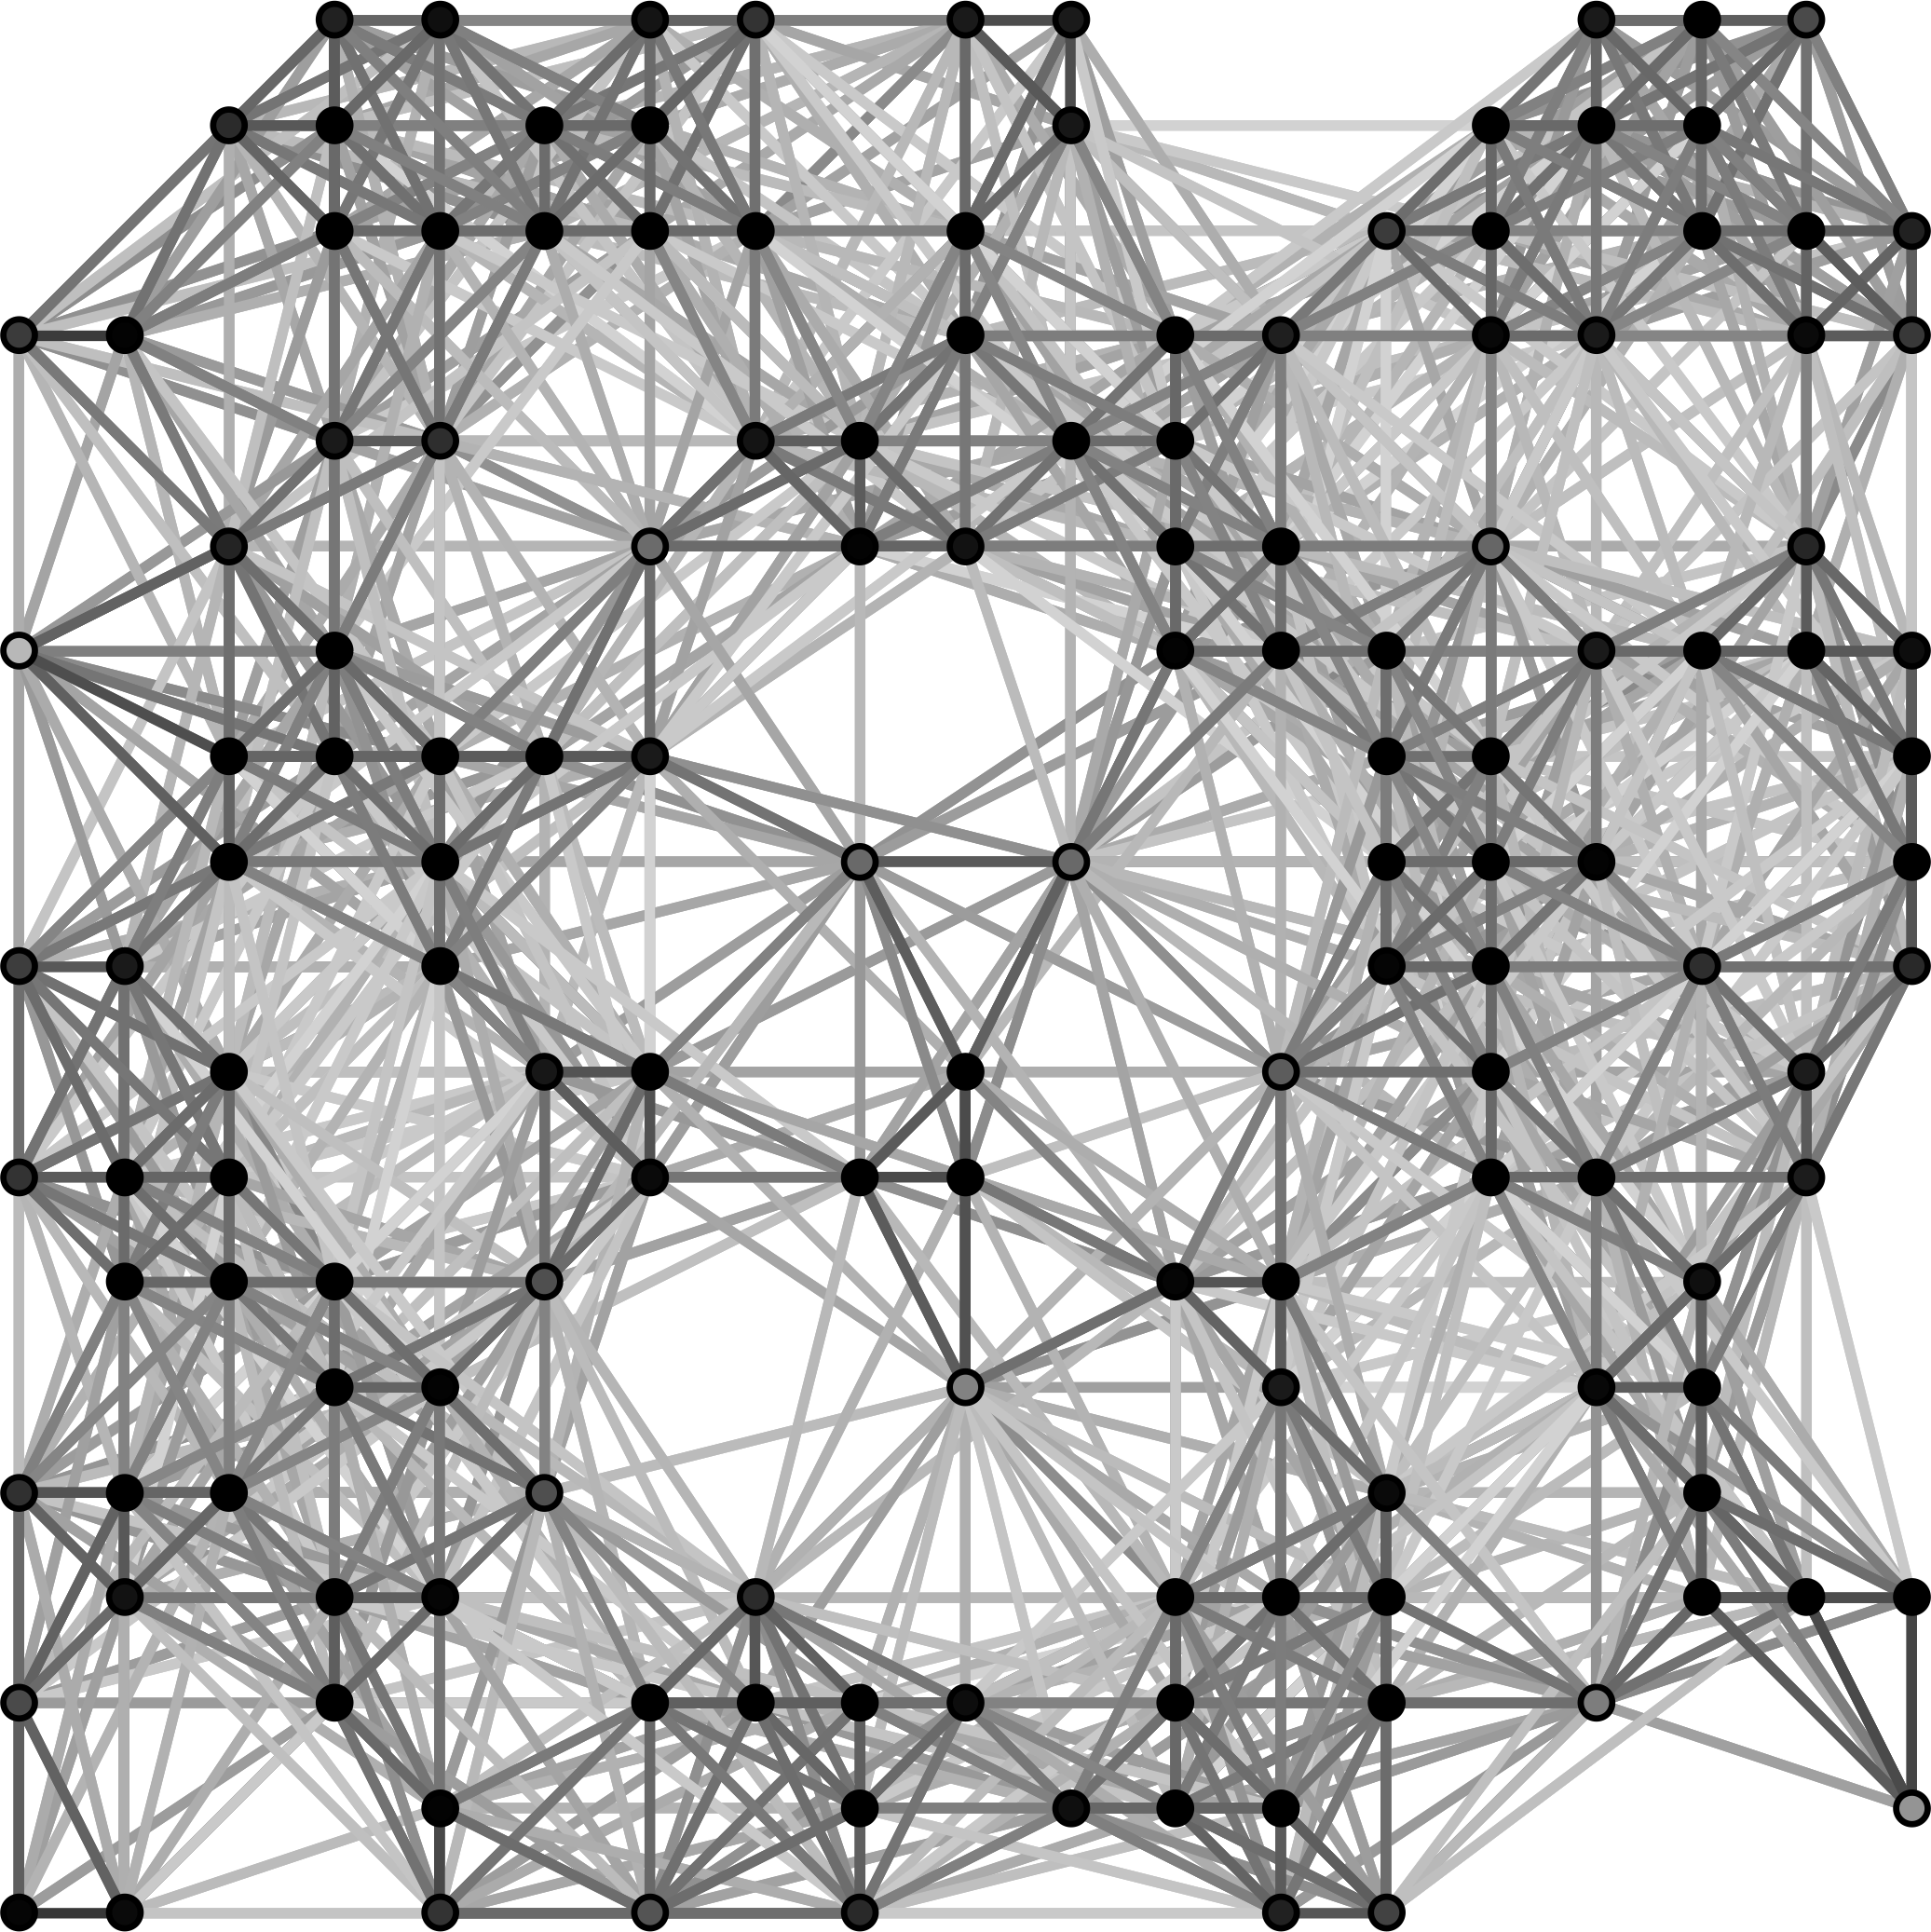
\includegraphics[width=\linewidth]{asset/mcl_iter_1.png}
    \subcaption{The graph with transition matrix \(\mathcal{M}^{(1)}\) after iteration 1.}
    \label{fig:mcl_iter_2}
  \end{subfigure}
  \hspace{0.5cm}

  \vspace{0.4cm}

  \hspace{0.5cm}
  \begin{subfigure}{0.40\linewidth}
    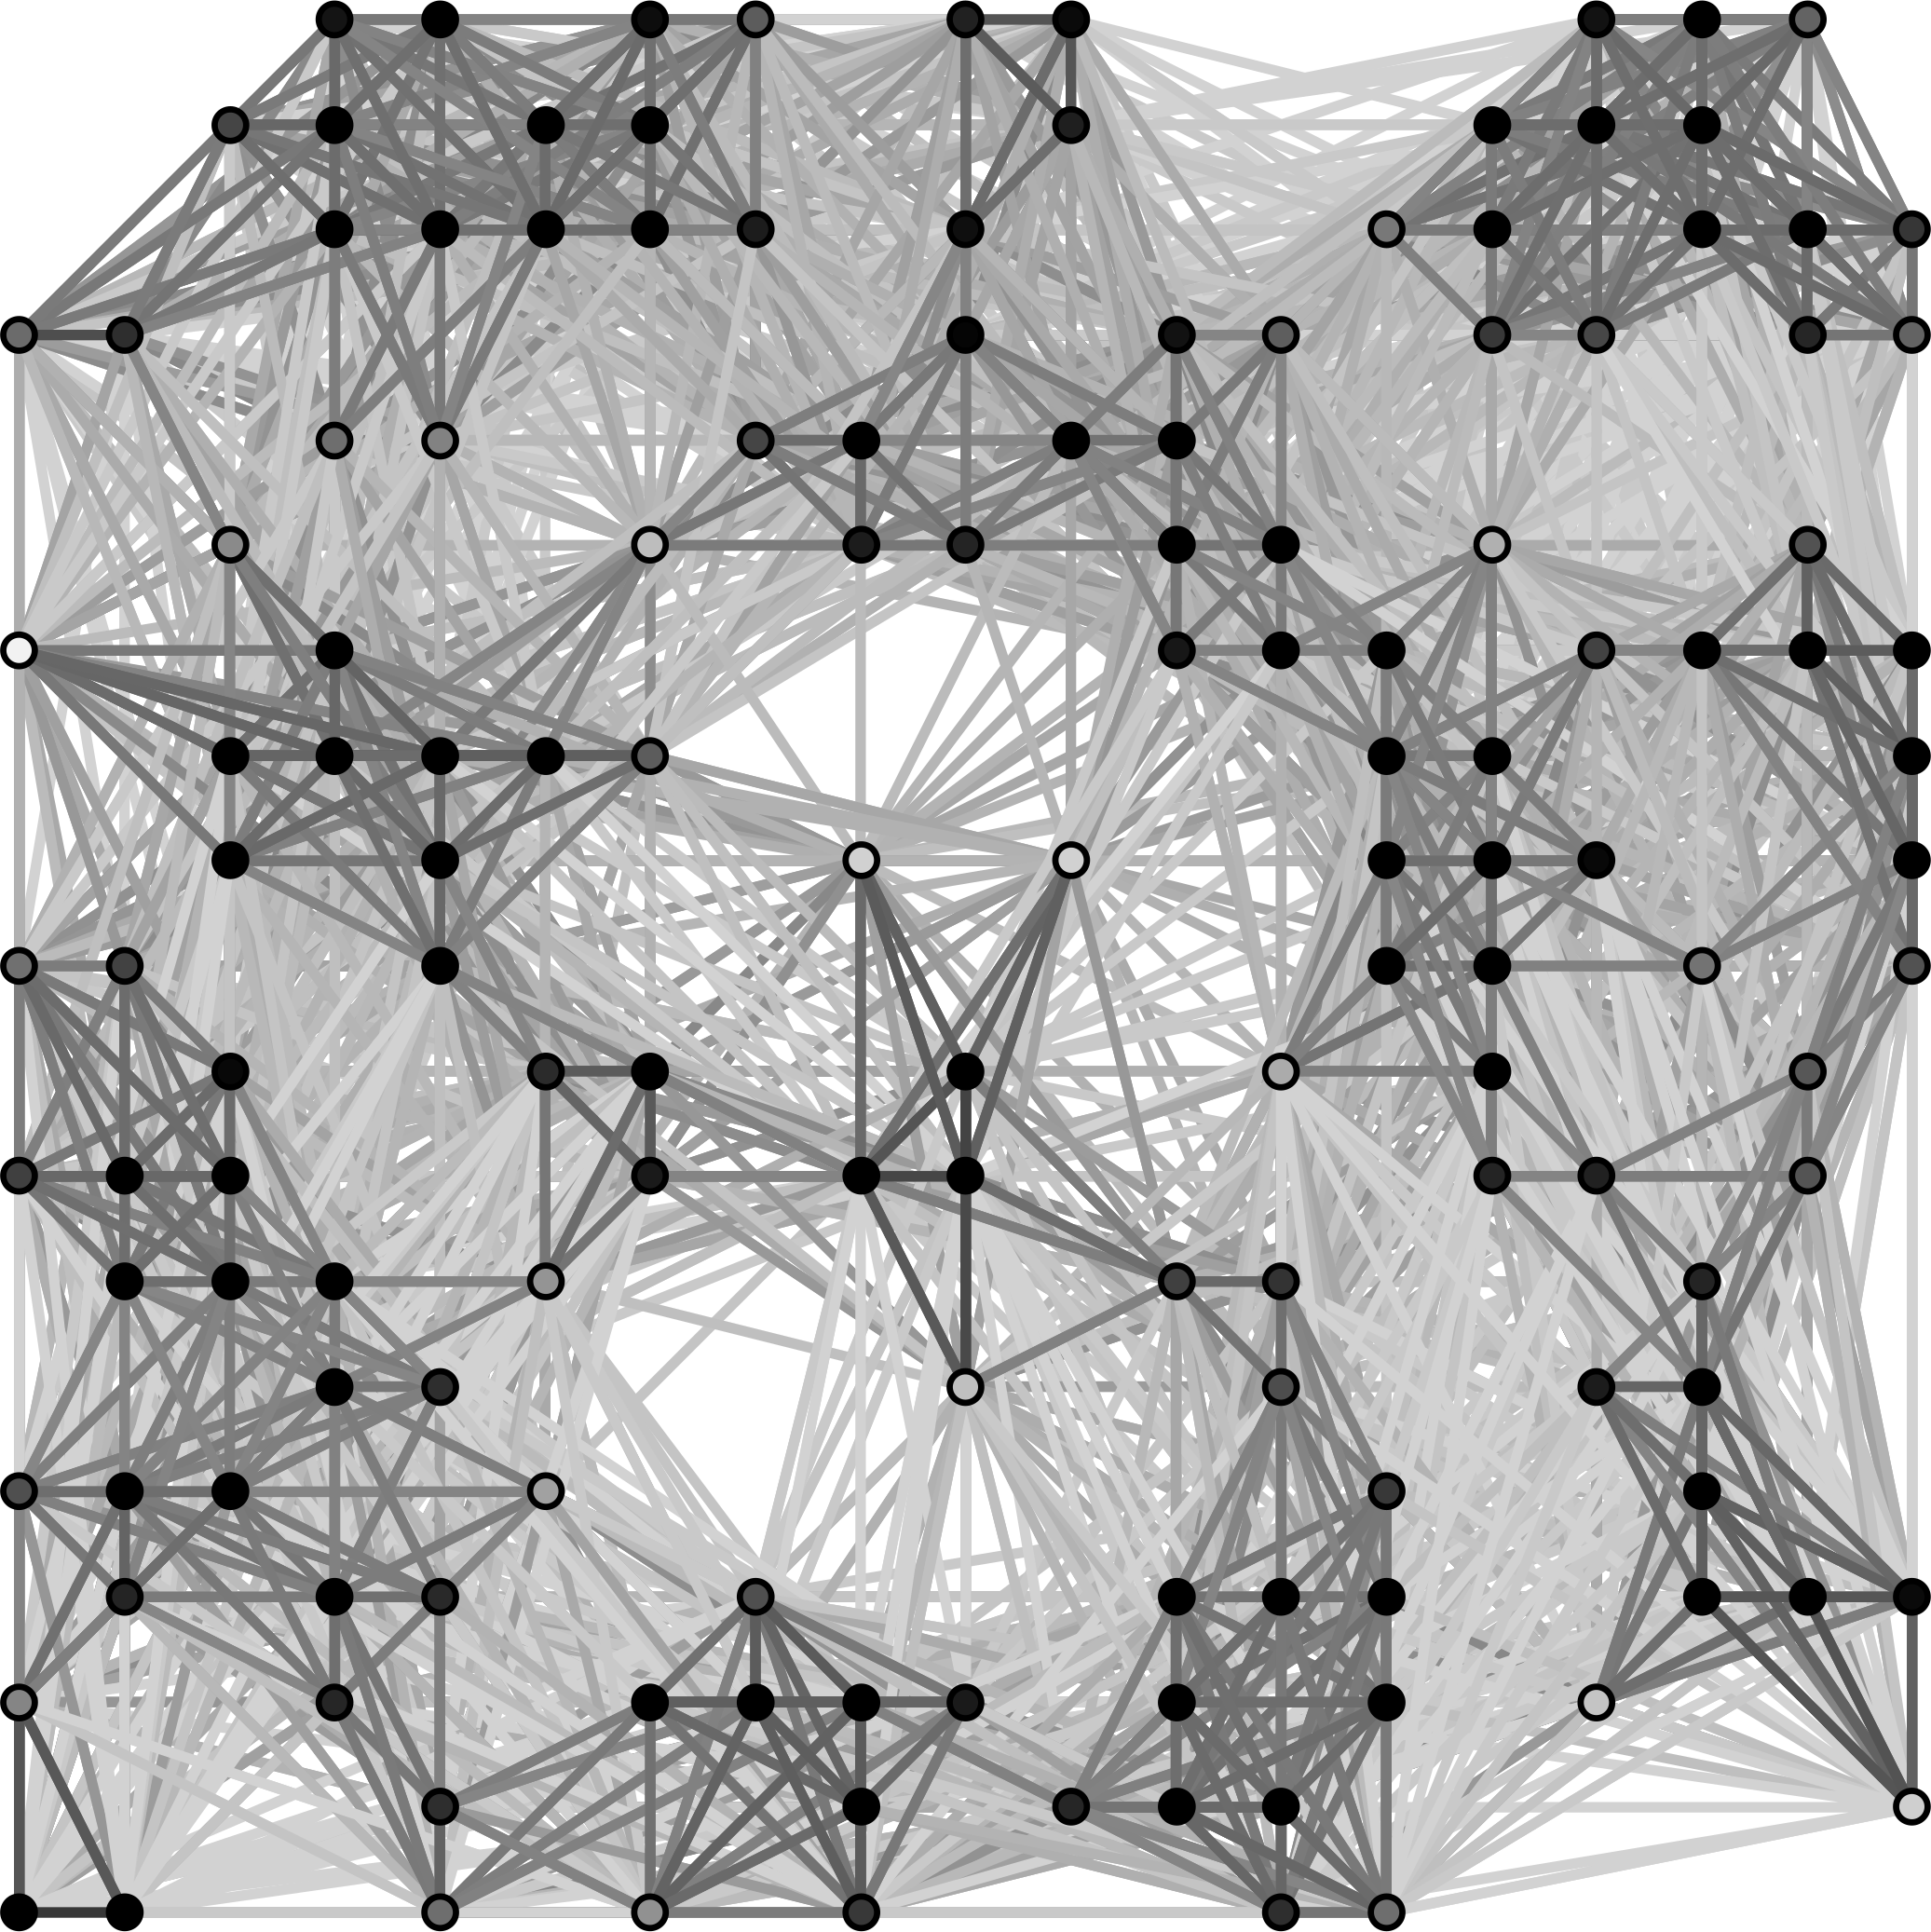
\includegraphics[width=\linewidth]{asset/mcl_iter_2.png}
    \subcaption{Transition matrix \(\mathcal{M}^{(2)}\) after iteration 2.}
    \label{fig:mcl_iter_3}
  \end{subfigure}
  \hfill
  \begin{subfigure}{0.40\linewidth}
    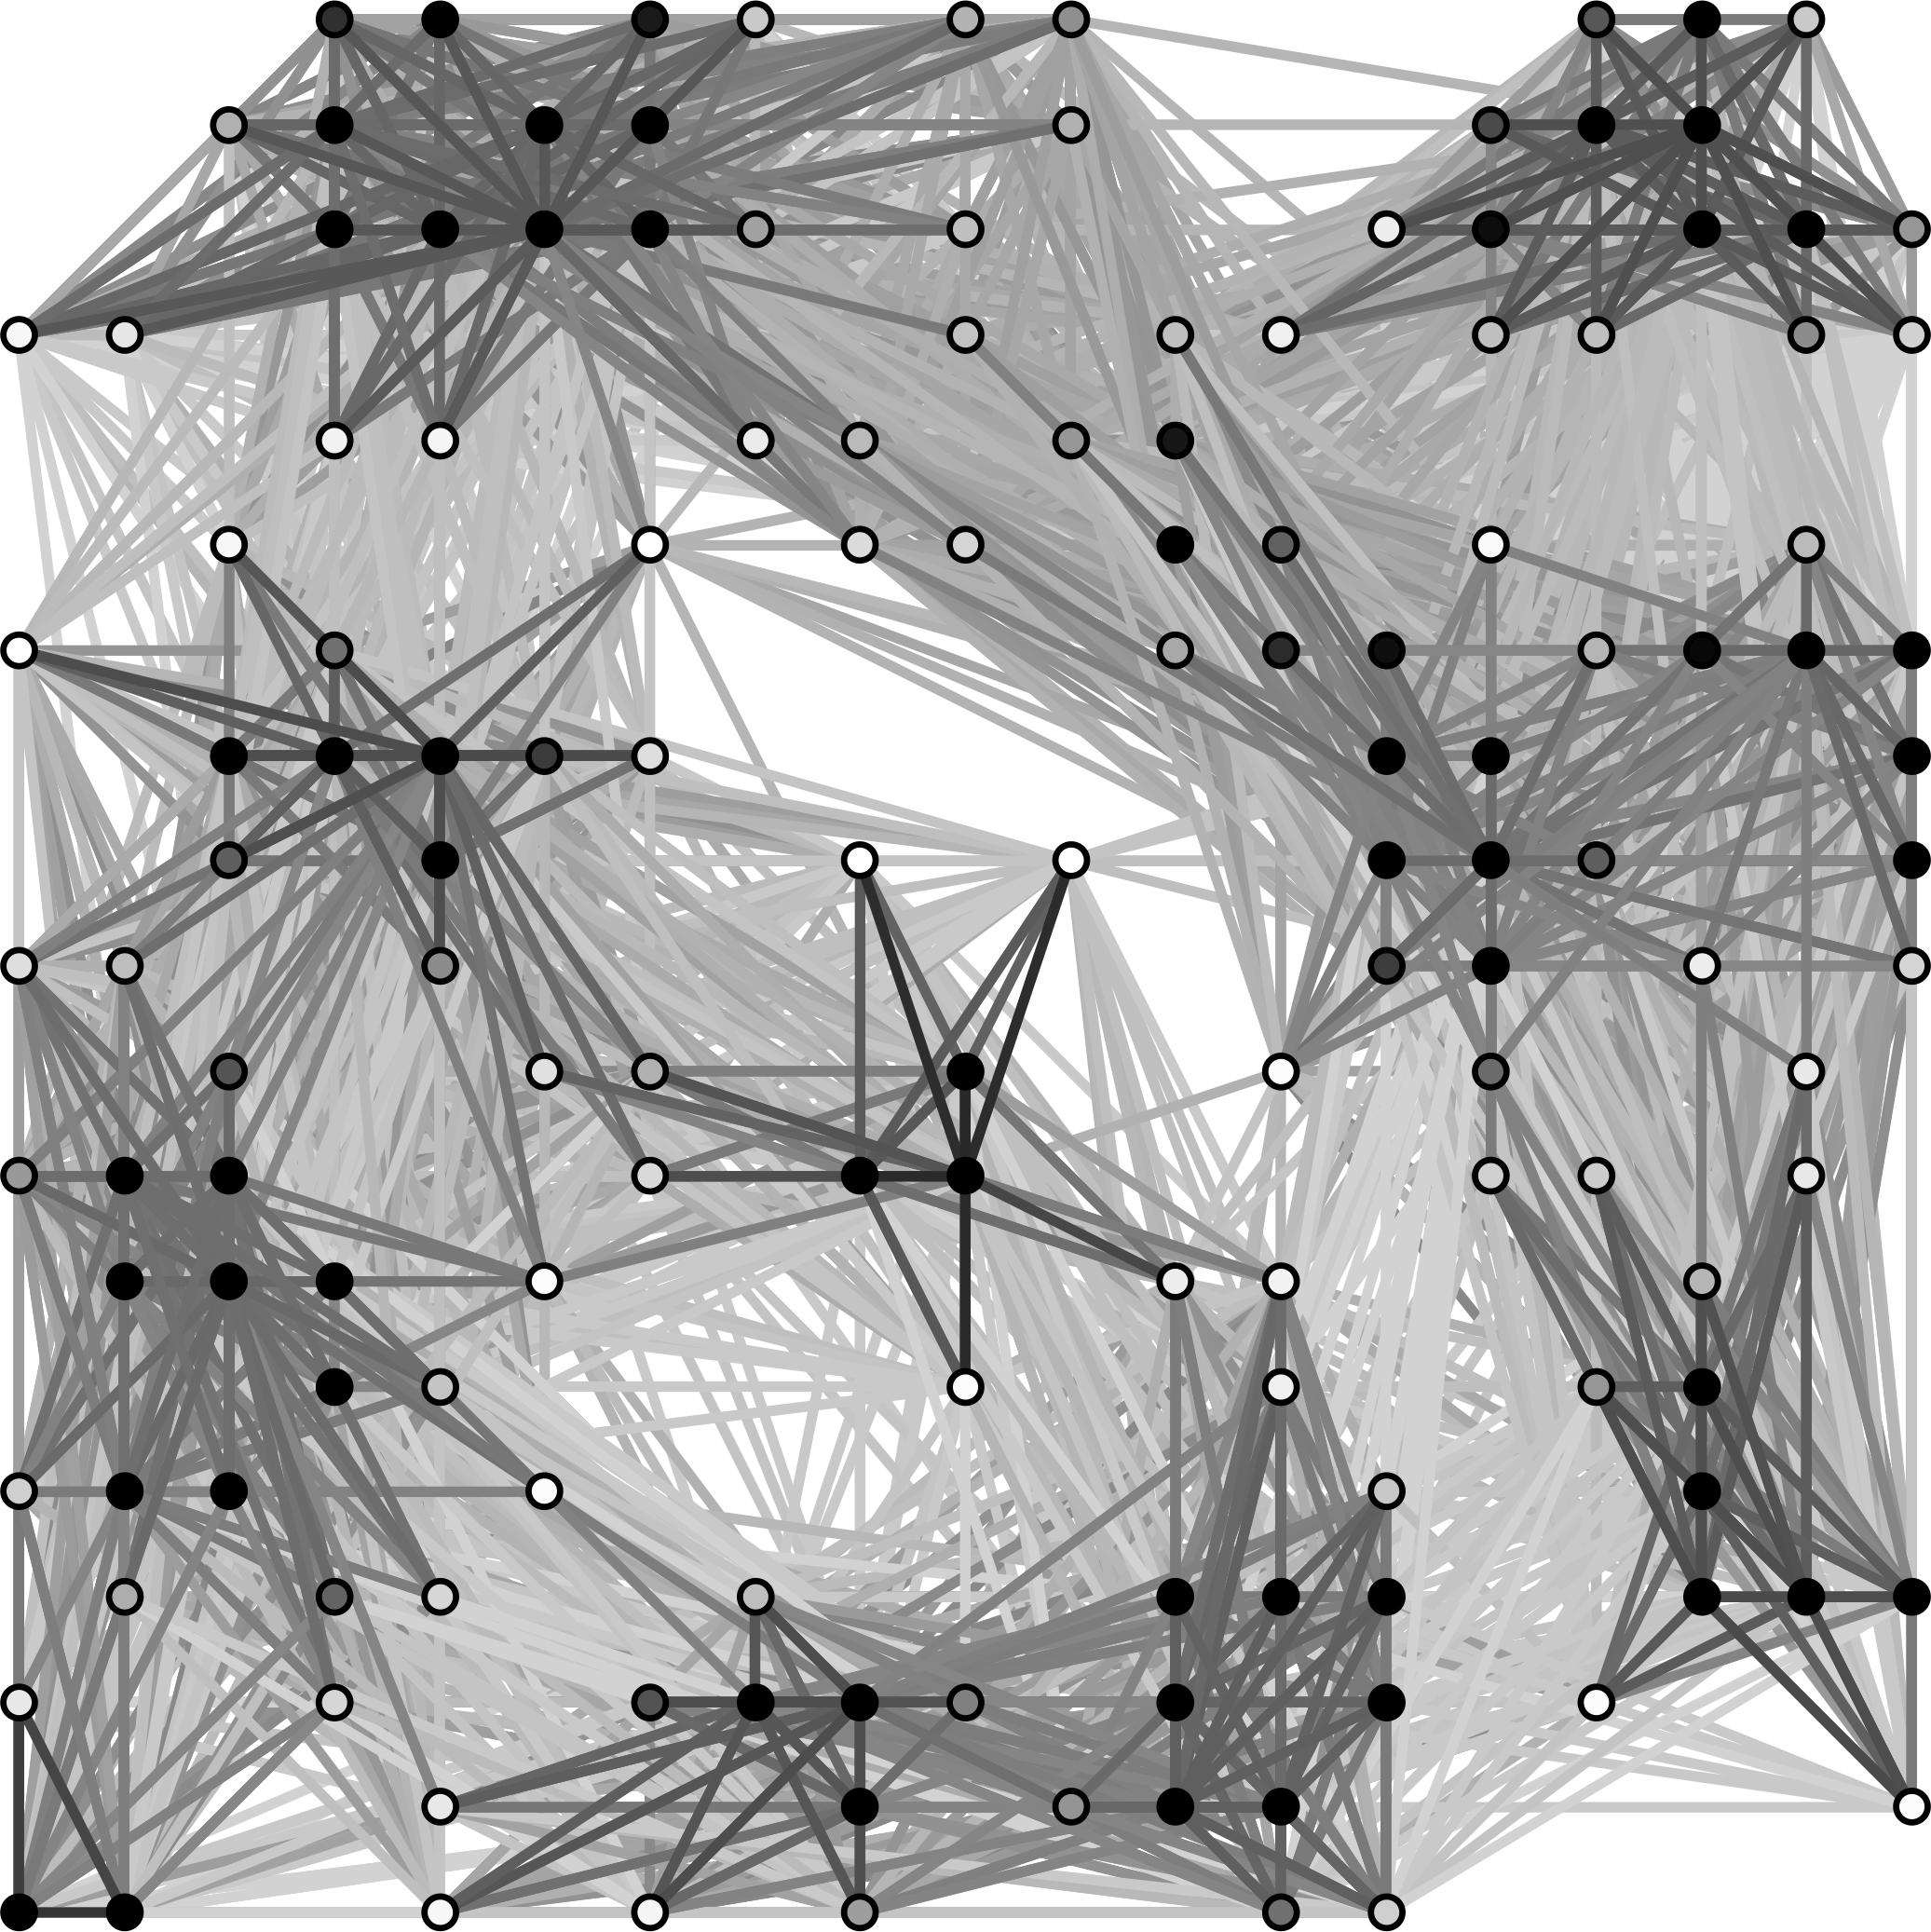
\includegraphics[width=\linewidth]{asset/mcl_iter_3.png}
    \subcaption{Transition matrix \(\mathcal{M}^{(3)}\) after iteration 3.}
    \label{fig:mcl_iter_4}
  \end{subfigure}
  \hspace{0.5cm}

  \vspace{0.4cm}

  \hspace{0.5cm}
  \begin{subfigure}{0.40\linewidth}
    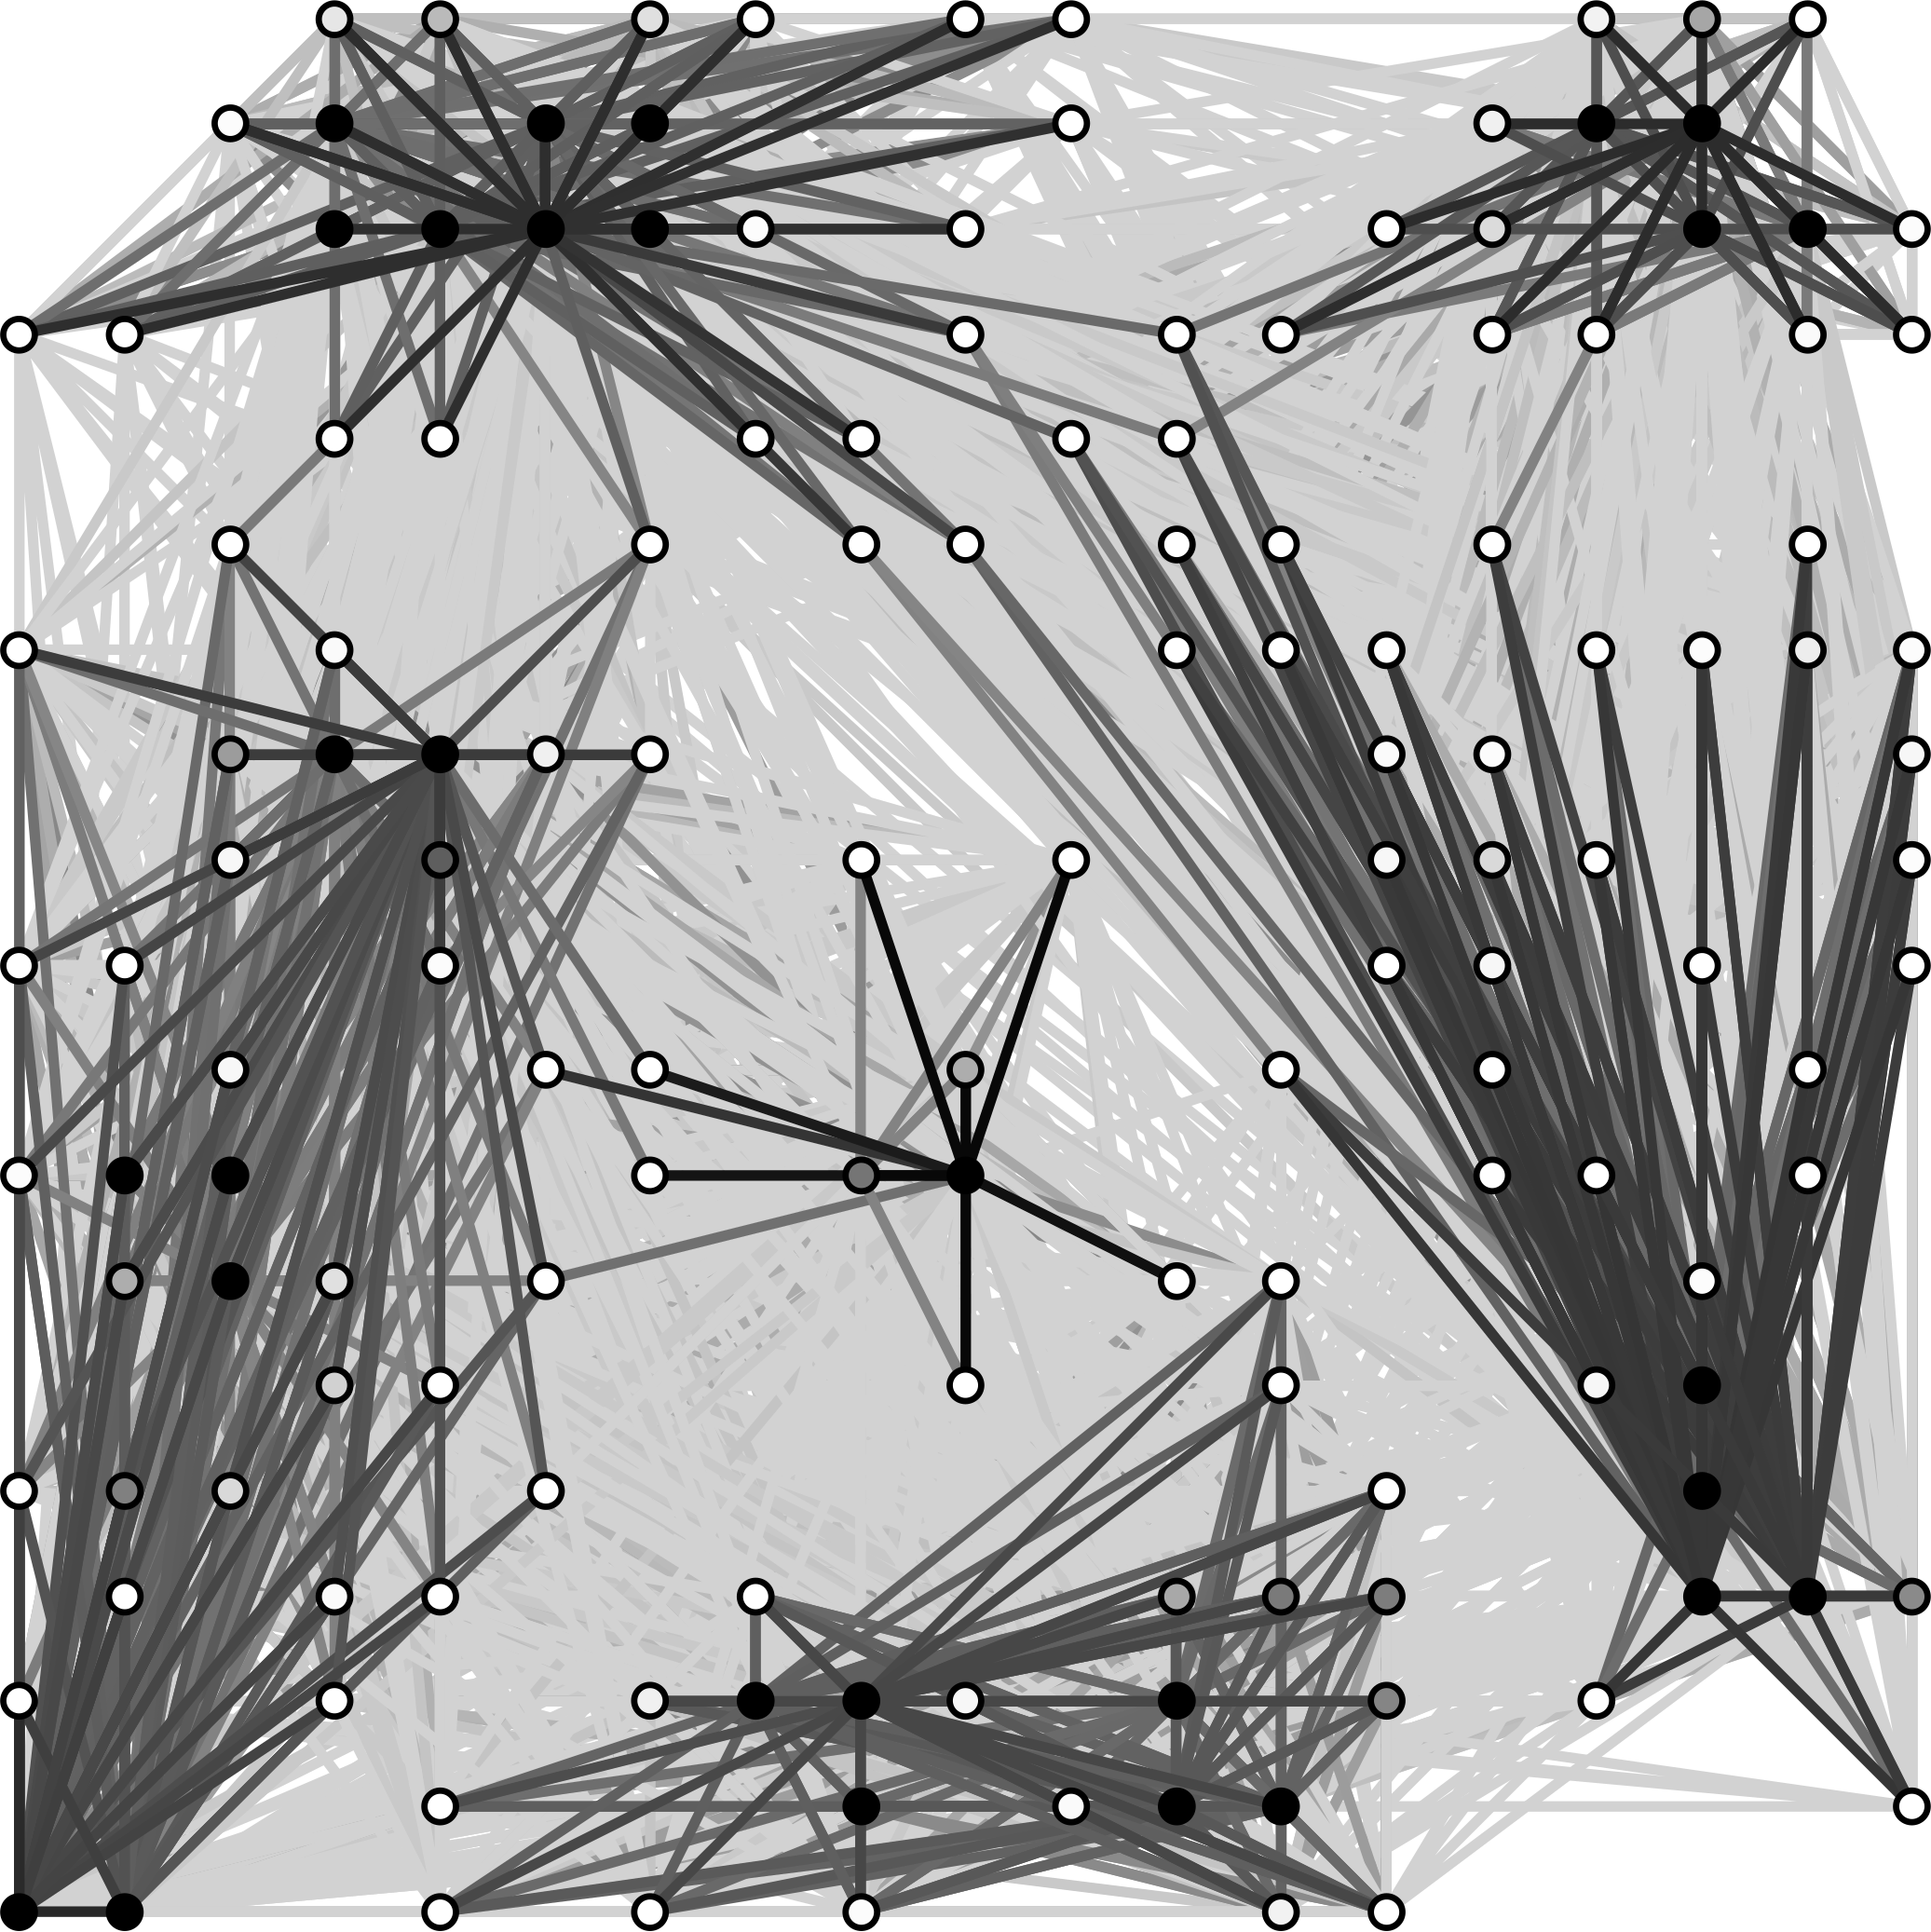
\includegraphics[width=\linewidth]{asset/mcl_iter_4.png}
    \subcaption{Transition matrix \(\mathcal{M}^{(4)}\) after iteration 4.\break}
    \label{fig:mcl_iter_5}
  \end{subfigure}
  \hfill
  \begin{subfigure}{0.40\linewidth}
    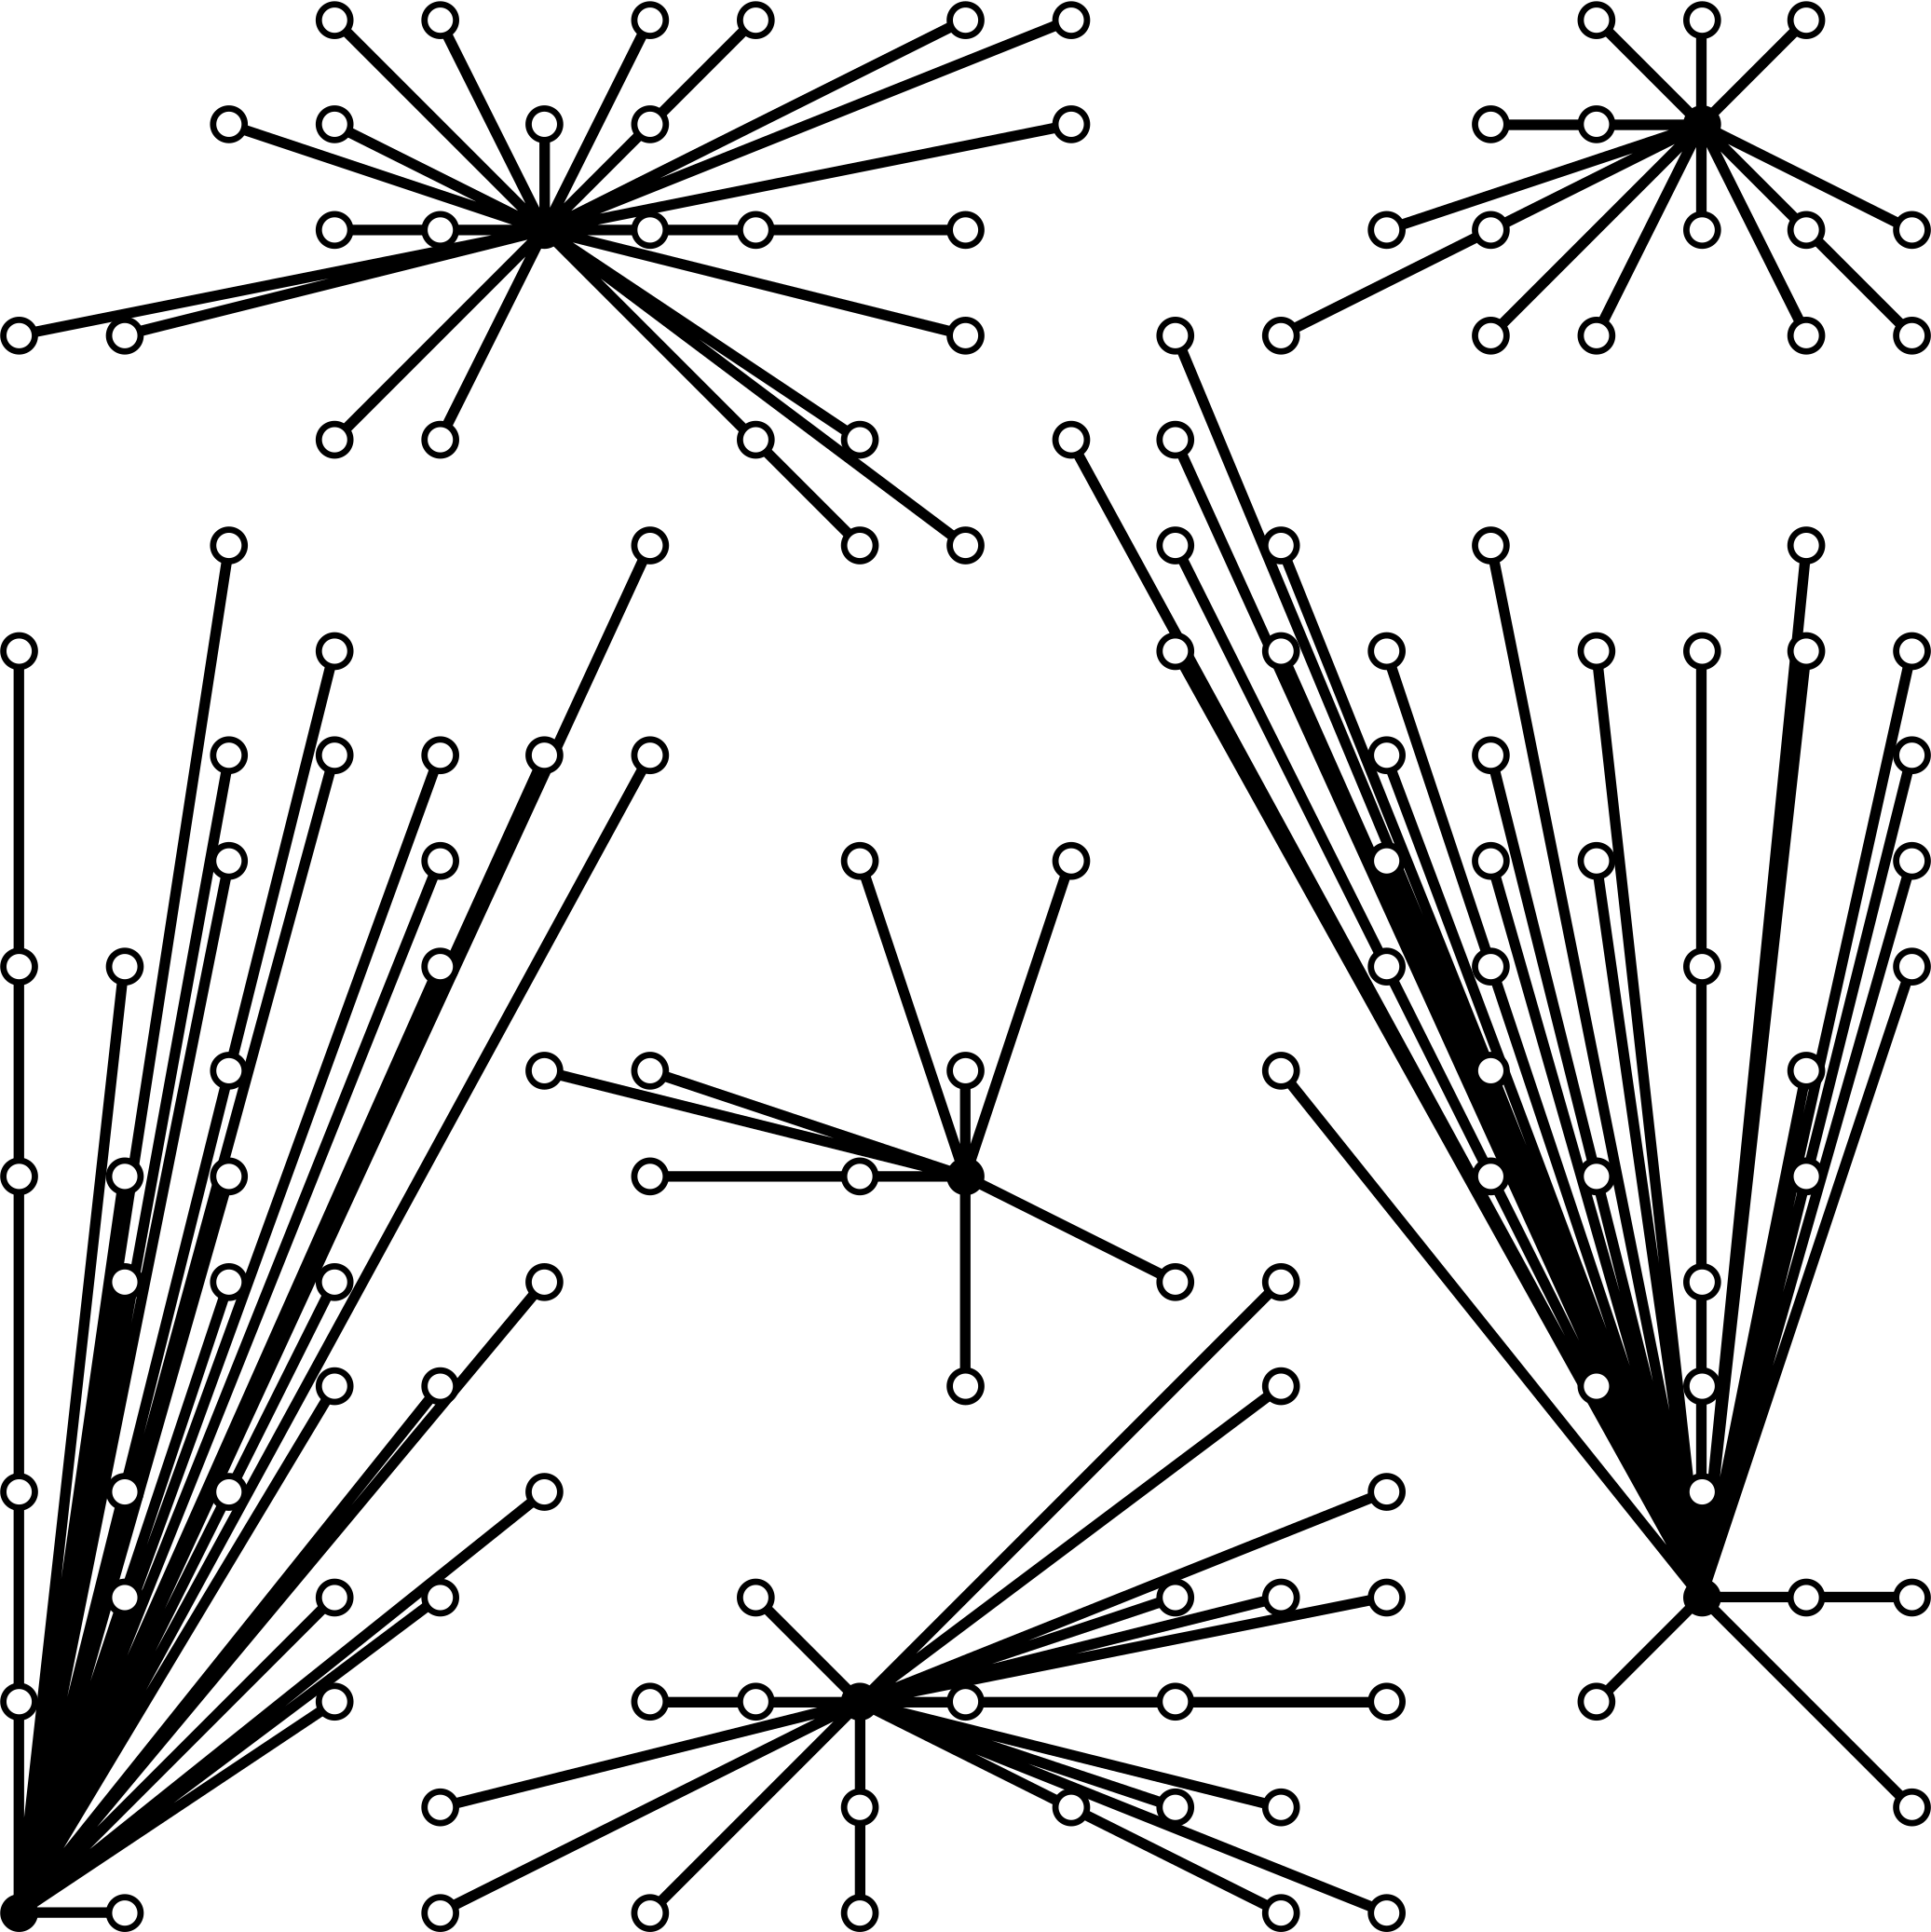
\includegraphics[width=\linewidth]{asset/mcl_iter_5.png}
    \subcaption{Converged transition matrix \(\lim_{\lambda \rightarrow \infty} \mathcal{M}^{(\lambda)}\). The cluster regions are apparent here.}
    \label{fig:mcl_iter_6}
  \end{subfigure}
  \hspace{0.5cm}

  \vspace{0.3cm}

  \caption{Source~\cite{mcl}. An intuitive demonstration of MCL applied on a sparse weighted graph. Each diagram is a depiction of the graph at different MCL iterations. The intensity of edge shades are proportional to the similarity or correlation of the linked vertex pair. Darker shades imply higher similarity, and conversely, lighter shades imply lower similarity.}
  \label{fig:mcl_iter}

\end{figure}

\subsection{Computational Overhead}

Like before, suppose that the transition matrix has shape \((n, n)\), while the
expansion parameter \(\epsilon\) is set to \(2\), a common design choice in MCL
literature. Each iteration consists of expansion (matrix squaring), pruning,
inflation, and normalization. For dense matrices, standard matrix
multiplication requires \(2 n^3 - n^2\) floating-point operations: each of the
\(n^2\) output entries requires \(n\) multiplications and \(n-1\) additions.
Inflation and normalization each contribute \(\mathcal{O}(n^2)\) operations;
specifically, inflation with non-integer exponent \(r>1\) costs
\(\sim 10 n^2\) FLOPs (assuming 10 FLOPs per elementwise exponentiation with
non-integer exponent), while normalization incurs \(n^2 - n\) FLOPs for column
sums and divisions. The termination criterion, evaluating the Frobenius norm
difference between successive matrices, adds roughly \(3n^2\) FLOPs per
iteration. Collectively, dense MCL requires \(\mathcal{O}(n^3)\) operations per
iteration, dominated by the expansion step, and consumes \(\mathcal{O}(n^2)\)
memory to store the full transition matrix. For example, given that each
element takes 32-bits, with \(10^5\) vertices in the graph, the memory reserved
for the transition matrix throughout the MCL runtime is \(\sim 37.25 \
\text{GiB}\). This renders dense MCL impractical for graphs with more than a frew thousand vertices, as the cubic growth quickly becomes prohivitive.
% Justification.
%\begin{align*}
%  (10^5)^2 \cdot 32 \ \text{bits} = 4 \cdot 10^{10} \ \text{bytes} = \dfrac{4 \cdot 10^{10}}{(2^{10})^3} \ \text{GiB} \approx 37.2529 \ \text{GiB}.
%\end{align*}

However, PSSNs are normally very sparse and this sparsity significantly reduces
the computational cost compared to \(\mathcal{O}(n^3)\) since operations
involving zero entries require no arithmetic operation and therefore take a
trivial number of cycles. This positive computational effect is reinforced by the pruning
operation at each subsequent MCL iteration. Therefore, we may accept that each column retains at most \(k_0: k_0 > 0\) non-zero
entries, where \(k_0\) can be influenced by the pruning threshold and is
typically much smaller than \(n\) in sparse PSSNs. Quantity \(k_0 \ll n\), often called
the \textit{average dimension}, determines the complexity of sparse operations.
For sparse matrices with average dimension \(k_0\), the computation of output column \(q\) is
\begin{align}
  \texttt{w}_{\cdot, q}^{(\lambda)}
  & = \mathcal{M}^{(\lambda-1)} \cdot \mathcal{M}^{(\lambda-1)}_{\cdot, q}
  \nonumber
  \\
  & = \sum_{k = 1}^{n} (\mathcal{M}^{(\lambda-1)}_{\cdot, k} \cdot \mathcal{M}^{(\lambda-1)}_{k, q})
  \nonumber
  \\
  & = \sum_{k = 1}^{k_0} (\mathcal{M}^{(\lambda-1)}_{\cdot, \xi_k} \cdot \mathcal{M}^{(\lambda-1)}_{\xi_k, q}).
  \label{eq:sparseExpansionCol}
\end{align}

The total number of elementary, non-zero computations becomes apparent in Eq~\ref{eq:sparseExpansionCol}. On that basis, the computation of each output column costs
\[
  \underbrace{k_0^2}_{\text{\# of multiplications}} + \ \ \ \ \underbrace{k_0 \cdot (k_0 - 1)}_{\text{\# of additions}} \ \ \text{FLOPs} = 2k_0^2 - k_0 \ \text{FLOPs}.
\]
This cost is repeated over all output columns \(n\). As a result, expansion
requires \(\mathcal{O}(n k_0^2)\) operations in total, while pruning,
inflation, and normalization each requires \(\mathcal{O}(n k_0)\) operations,
reducing the overall computational requirement down to \(\mathcal{O}(n
k_0^2)\). Memory consumption is also reduced down to \(\mathcal{O}(n k_0)\)
since the transition matrix may be stored in a compressed sparse format.
Fig.~\ref{fig:complexity} highlights the complexity advantage for
representative \(k_0\) values.

\begin{figure}[htbp]
  \centering
  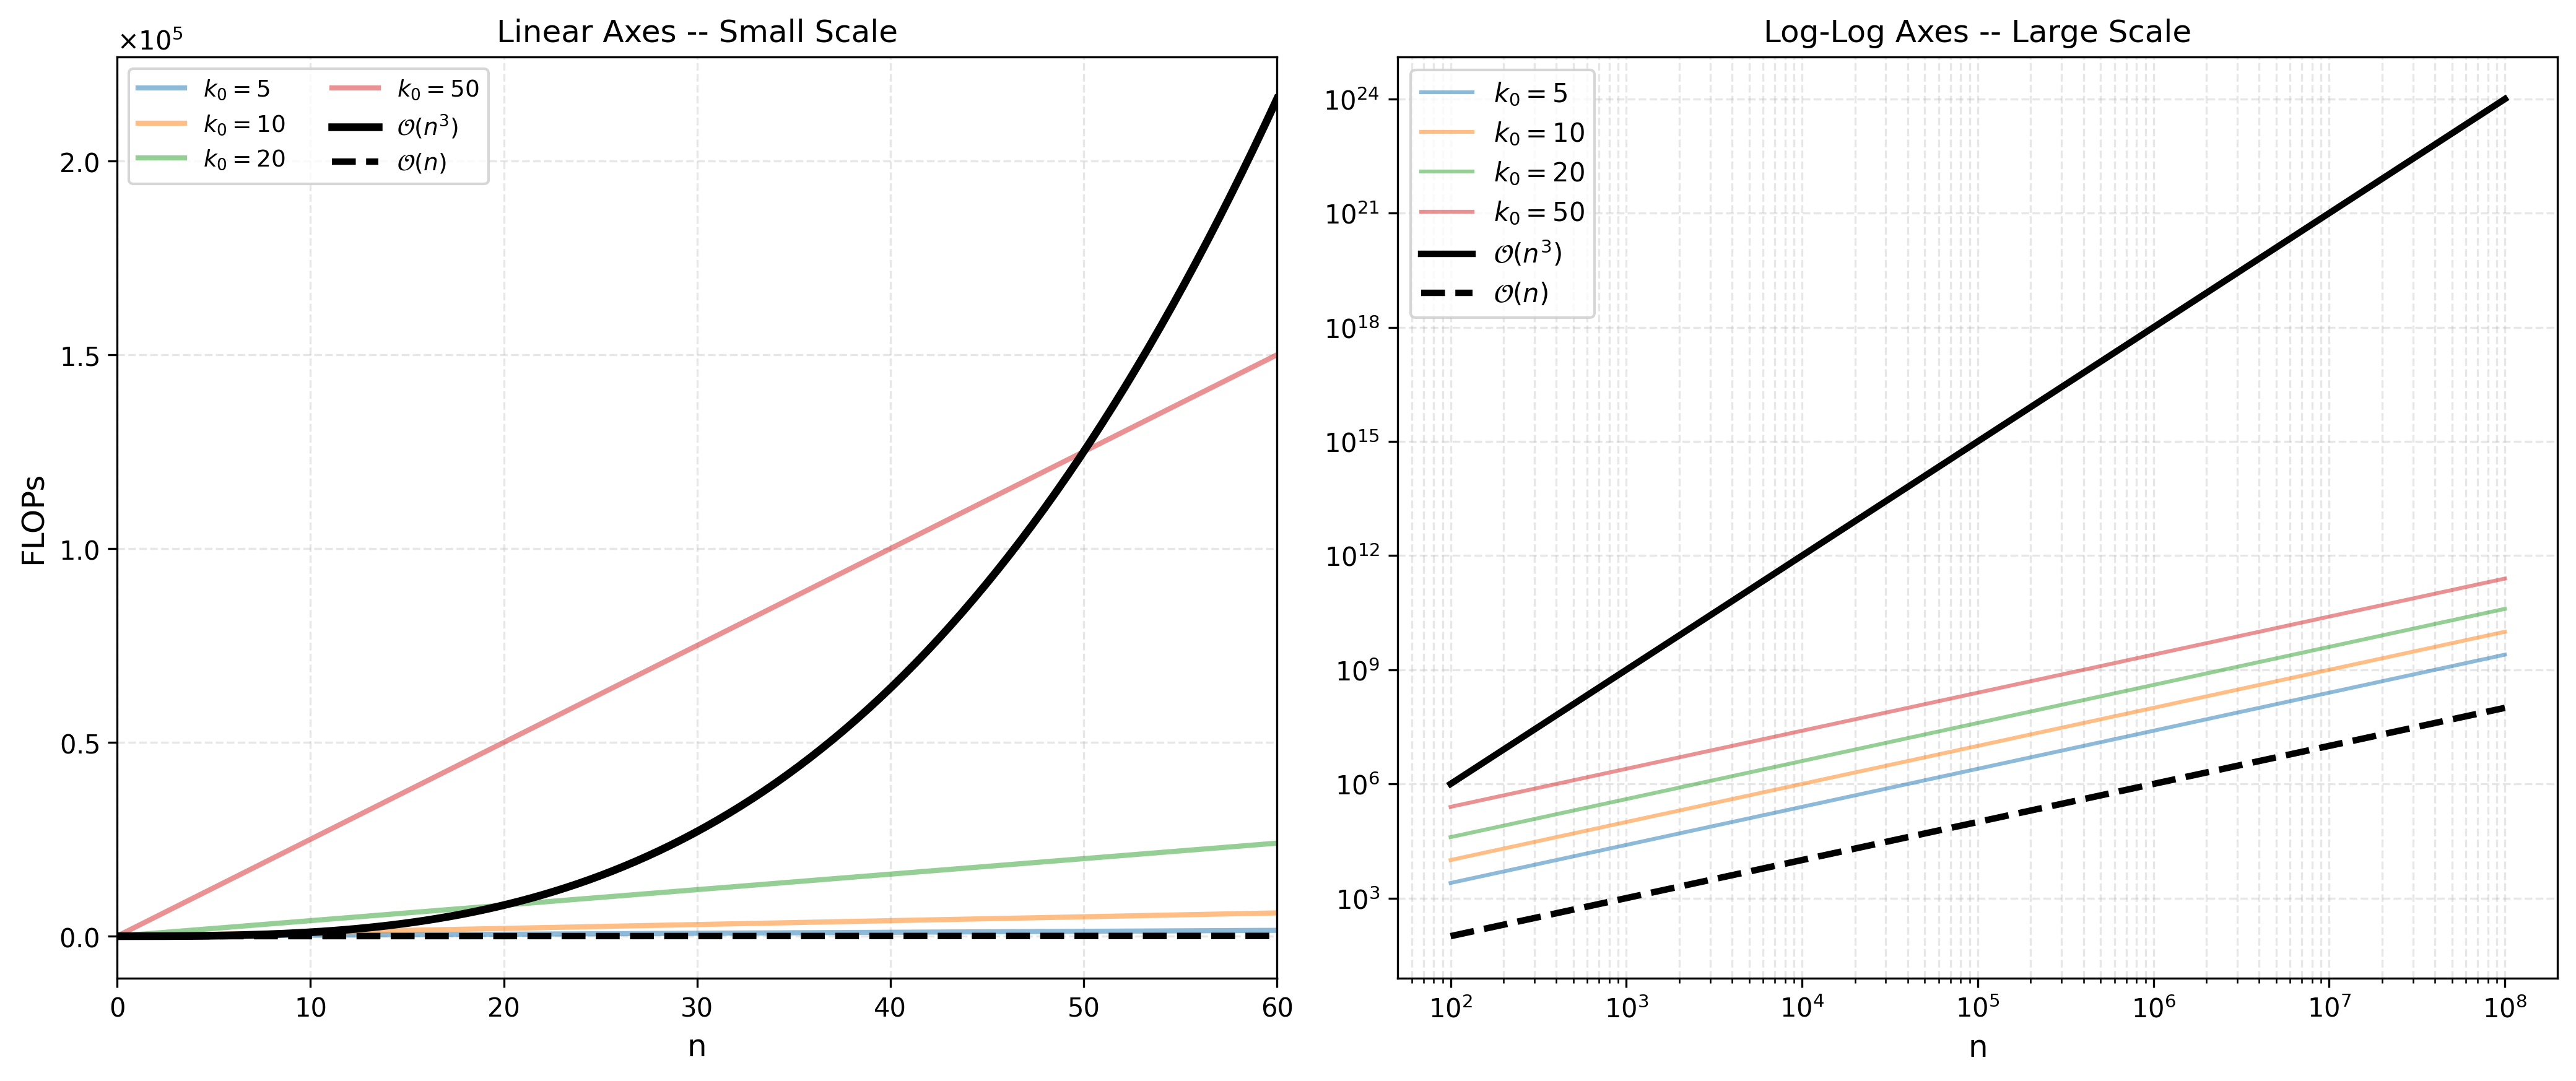
\includegraphics[width=1\linewidth]{asset/complexity.png}
  \caption{Complexity of sparse expansion \(\mathcal{O}(n k_0^2)\)
  compared against dense for \(k_0 \in \{5, 10, 20, 50 \}\) shown in color. The
  left plot uses linear axes to emphasize curvature at small \(n\), while the
  right plot uses log-log (base \(10\)) axes to illustrate scaling across many
  orders of magnitude.}
  \label{fig:complexity}
\end{figure}

Thus, in the numerical example where we assumed \(10^5\) vertices, if we
impose that only \(1 \%\) of the edges are non-zero, then the average
dimension \(k_0\) is \(10^3\). Therefore, the entire graph can be compressed
to an object reserving \(\sim 372.5 \ \text{MiB} \ll 37.25 \ \text{GiB}\)
which is a huge improvement when compared to the previous unoptimized
approach.
